\documentclass[letterpaper,12pt]{article}

% --- PAQUETES DE IDIOMA
\usepackage[spanish,mexico]{babel}
\usepackage[utf8]{inputenc}
\usepackage{csquotes}

\usepackage[utf8]{inputenc}
\usepackage[T1]{fontenc}
% --- PAQUETES MATEMÁTICOS --
\usepackage{amsmath}
\usepackage{amssymb}
\usepackage{cancel}
\usepackage{mathrsfs}

% --- PAQUETES GRÁFICOS Y DE DISEÑO ---
\usepackage{graphicx}
\usepackage{float}
\usepackage{subcaption}
\usepackage[table]{xcolor}
\usepackage{longtable}
\usepackage{multirow}
\usepackage{makecell}
\usepackage{array}
\usepackage{caption}
\usepackage{tikz}
\usetikzlibrary{decorations.pathreplacing}
\usetikzlibrary{decorations.pathmorphing}
\usepackage{circuitikz}
\usetikzlibrary{shapes.geometric, shapes.multipart, shapes.symbols, positioning, arrows.meta, calc, shadows, decorations.pathreplacing,babel}

% --- LISTAS ---
\usepackage{enumitem}

% --- PAQUETES DE CÓDIGO ---
\usepackage{listings}
% Configuración del estilo de listings
\definecolor{codebg}{rgb}{0.95,0.95,0.95}   
\definecolor{keyword}{rgb}{0.0,0.2,0.6}     
\definecolor{comment}{rgb}{0.25,0.5,0.35}   
\definecolor{string}{rgb}{0.6,0.0,0.0}      
\definecolor{number}{rgb}{0.5,0.0,0.5}      
\definecolor{codegray}{rgb}{0.5,0.5,0.5}
\definecolor{codepurple}{rgb}{0.58,0,0.82}
\definecolor{backcolour}{rgb}{0.95,0.95,0.95}


% Colores para la Tabla 10-2
\definecolor{headerBlueA}{RGB}{91, 155, 213}   % Azul medio para el encabezado
\definecolor{rowBlueA}{RGB}{233, 242, 250}    % Azul muy claro para la fila
\definecolor{borderBlueA}{RGB}{156, 194, 229} % Azul claro para los bordes

% Colores para la Tabla 10-1
\definecolor{headerBlueB}{RGB}{68, 114, 196}  % Azul oscuro para el encabezado
\definecolor{rowBlueB}{RGB}{217, 225, 242}    % Azul claro para filas intercaladas
\definecolor{borderBlueB}{RGB}{143, 170, 220} % Azul medio para los bordes

% Colores para la Tabla 8-2 (Amarillo/Oro)
\definecolor{hdryellow}{RGB}{255, 192, 0}
\definecolor{row1yellow}{RGB}{255, 242, 204}
\definecolor{row2yellow}{RGB}{255, 249, 227}

% Definición de los colores utilizados en las tablas
\definecolor{headerbg}{HTML}{5B84C4} % Azul oscuro para el encabezado principal
\definecolor{subheaderbg}{HTML}{B4C6E7} % Azul intermedio para sub-encabezados
\definecolor{rowbg}{HTML}{E9EDF4} % Azul claro para filas intercaladas

% Definición de colores exactos para las tablas y semáforo
\definecolor{SemGreen}{RGB}{0, 176, 80}
\definecolor{SemYellow}{RGB}{255, 255, 0}
\definecolor{SemRed}{RGB}{255, 0, 0}

\definecolor{TabOrangeHead}{RGB}{237, 125, 49}
\definecolor{TabOrangeBody}{RGB}{252, 228, 214}

\definecolor{TabGreyHead}{RGB}{165, 165, 165}
\definecolor{TabGreyBody}{RGB}{237, 237, 237}

\definecolor{TabBlueHead}{RGB}{68, 114, 196}
\definecolor{TabBlueBody}{RGB}{217, 225, 242}

\definecolor{keywords}{RGB}{128,0,128}    % Morado para palabras clave
\definecolor{numbers}{RGB}{205,92,92}     % Naranja/Rojo para números
\definecolor{strings}{RGB}{34,139,34}     % Verde para texto
\definecolor{comments}{RGB}{169,169,169}  % Gris para comentarios
\definecolor{background}{RGB}{252,252,252}% Fondo muy claro

\lstset{
    language=Python,
    backgroundcolor=\color{background},
    basicstyle=\ttfamily\normalsize,
    keywordstyle=\color{keywords}\bfseries,
    stringstyle=\color{strings},
    commentstyle=\color{comments}\itshape,
    numberstyle=\color{numbers},
    % Añadir palabras de MicroPython a las keywords
    morekeywords={Pin, I2C, freq, readfrom, from_bytes, hex, range, sleep, scan, port, pin, putstr, clear, move_to, show, text, round, sleep_ms, utime, True, False},
    % Colorear los números
    literate=
        {0}{{{\color{numbers}0}}}1
        {1}{{{\color{numbers}1}}}1
        {2}{{{\color{numbers}2}}}1
        {3}{{{\color{numbers}3}}}1
        {4}{{{\color{numbers}4}}}1
        {5}{{{\color{numbers}5}}}1
        {6}{{{\color{numbers}6}}}1
        {7}{{{\color{numbers}7}}}1
        {8}{{{\color{numbers}8}}}1
        {9}{{{\color{numbers}9}}}1
        {0x39}{{{\color{numbers}0x39}}}4
        {0x3F}{{{\color{numbers}0x3F}}}4
        {0x3E}{{{\color{numbers}0x3E}}}4
        {0x27}{{{\color{numbers}0x27}}}4
        {0x48}{{{\color{numbers}0x48}}}4,
    showstringspaces=false,
    breaklines=true,
    frame=none,
    numbers=none,
    tabsize=4,
    belowcaptionskip=1em,
    abovecaptionskip=1em
}

\lstset{
  backgroundcolor=\color{backcolour},
  basicstyle=\ttfamily\small,
    inputencoding=utf8,
  keywordstyle=\color{blue}\bfseries,
  stringstyle=\color{codepurple},
  commentstyle=\color{codegray}\itshape,
  numbers=left,
  numberstyle=\tiny\color{codegray},
  frame=single,
  rulecolor=\color{black},
  breaklines=true,
  tabsize=4,
  showstringspaces=false,
  extendedchars=true,
  literate={á}{{\'a}}1
           {é}{{\'e}}1
           {í}{{\'i}}1
           {ó}{{\'o}}1
           {ú}{{\'u}}1
           {Á}{{\'A}}1
           {É}{{\'E}}1
           {Í}{{\'I}}1
           {Ó}{{\'O}}1
           {Ú}{{\'U}}1
           {ñ}{{\~n}}1
           {Ñ}{{\~N}}1
           {¿}{{\textquestiondown}}1
           {¡}{{\textexclamdown}}1
           {°}{{\textdegree}}1
           {ø}{{\o}}1
}

% Definición del lenguaje Python para listings
\lstdefinelanguage[LAB]{Python}{
    morekeywords={False, None, True, and, as, assert, async, await, break,
                                class, continue, def, del, elif, else, except, finally,
                                for, from, global, if, import, in, is, lambda, nonlocal,
                                not, or, pass, raise, return, try, while, with, yield,
                                machine, Pin, PWM, ADC, Timer, sleep_ms, sleep_us},
    morecomment=[l]{\#},
    morestring=[b]",
    morestring=[b]',
    sensitive=true
}

% --- ESTILOS PARA DIAGRAMAS DE FLUJO (TIKZ) ---
\tikzset{
  startstop/.style={rectangle, rounded corners, minimum width=3cm, minimum height=1cm, align=center, draw=black, fill=red!30},
  process/.style={rectangle, minimum width=3cm, minimum height=1cm, align=center, draw=black, fill=orange!30},
  decision/.style={diamond, aspect=2, minimum width=3cm, minimum height=1cm, align=center, draw=black, fill=green!30},
  io/.style={trapezium, trapezium left angle=70, trapezium right angle=110, minimum width=3cm, minimum height=1cm, align=center, draw=black, fill=blue!30},
  arrow/.style={thick,->,>=stealth}
}

% Definimos el color dorado/naranja para el cuadro de texto
\definecolor{goldbox}{RGB}{218, 140, 15}

% Macro para dibujar la Raspberry Pi Pico y sus nodos
\newcommand{\picoboard}{
    \draw[thick] (0,0.5) rectangle (4,-9.5);
    \node[align=center, font=\small\sffamily] at (2, -1.5) {Raspberry PI\\[0.1cm]Pico};

    % Pines Superiores
    \draw[red, thick] (0.8, 0.5) -- (0.8, 0.8) coordinate (P41); \node[above, font=\tiny\sffamily, inner sep=1pt] at (P41) {41};
    \draw[red, thick] (2.0, 0.5) -- (2.0, 0.8) coordinate (P42); \node[above, font=\tiny\sffamily, inner sep=1pt] at (P42) {42};
    \draw[red, thick] (3.2, 0.5) -- (3.2, 0.8) coordinate (P43); \node[above, font=\tiny\sffamily, inner sep=1pt] at (P43) {43};
    \node[below, font=\tiny\sffamily] at (0.8, 0.5) {SW CLK};
    \node[below, font=\tiny\sffamily] at (2.0, 0.5) {SW GND};
    \node[below, font=\tiny\sffamily] at (3.2, 0.5) {SW DIO};

    % GND Inferior
    \draw[red, thick] (2, -9.5) -- (2, -10.2) coordinate (PGND);
    \node[above, font=\tiny\sffamily] at (2, -9.5) {GND};
    \node[below, font=\tiny\sffamily] at (2, -10.2) {3,8,13,18 \quad 23,28,38};

    % Pines del lado Izquierdo
    \foreach \i/\pin/\num in {
        1/GP0/1, 2/GP1/2, 
        4/GP2/4, 5/GP3/5, 6/GP4/6, 7/GP5/7, 
        9/GP6/9, 10/GP7/10, 11/GP8/11, 12/GP9/12, 
        14/GP10/14, 15/GP11/15, 16/GP12/16, 17/GP13/17, 
        19/GP14/19, 20/GP15/20
    } {
        \draw[red, thick] (0, -\i*0.45) -- (-0.4, -\i*0.45) coordinate (P\num);
        \node[right, font=\tiny\sffamily] at (0, -\i*0.45) {\pin};
        \node[above left, font=\tiny\sffamily, inner sep=1pt] at (P\num) {\num};
    }

    % Pines del lado Derecho
    \foreach \i/\pin/\num in {
        1/VBUS/40, 2/VSS/39, 
        4/3V3\_EN/37, 5/3V3/36, 6/ADC\_VREF/35, 7/GP28\_A2/34, 8/AGND/33, 
        9/GP27\_A1/32, 10/GP26\_A0/31, 11/RUN/30, 12/GP22/29, 
        14/GP21/27, 15/GP20/26, 16/GP19/25, 17/GP18/24, 
        19/GP17/22, 20/GP16/21
    } {
        \draw[red, thick] (4, -\i*0.45) -- (4.4, -\i*0.45) coordinate (P\num);
        \node[left, font=\tiny\sffamily] at (4, -\i*0.45) {\pin};
        \node[above right, font=\tiny\sffamily, inner sep=1pt] at (P\num) {\num};
    }
}



\definecolor{azulresultado}{HTML}{0072C6}
\definecolor{rojoacarreo}{HTML}{FF0000}

% Colores para la tabla
\definecolor{headblue}{HTML}{4F81BD}
\definecolor{subheadblue}{HTML}{B8CCE4}
\definecolor{datablockblue}{HTML}{DCE6F1}
% Definición de los colores extraídos de la imagen
\definecolor{HeaderBlue}{RGB}{68, 114, 196}  % Azul fuerte del encabezado
\definecolor{RowBlue}{RGB}{217, 225, 242}    % Azul claro de la primera fila
\definecolor{BorderBlue}{RGB}{143, 172, 223} % Azul medio para los bordes

% --- RUTAS DE IMÁGENES ---
\graphicspath{{img/}{portada_img/}}

\definecolor{armblue}{RGB}{0, 113, 188}

% --- CONFIGURACIÓN DE PÁGINA (GEOMETRÍA) ---
\usepackage[
    left=25mm, 
    right=25mm,
    top=35mm,
    bottom=30mm,
    headheight=77pt, 
    papersize={21.59cm,27.94cm}
]{geometry}

% --- FORMATO DE TEXTO ---
\renewcommand{\baselinestretch}{1.25} 
\usepackage{parskip} 
\usepackage{lipsum}  

% --- VARIABLES GLOBALES ---
\newcommand{\materia}{}

% --- ENCABEZADOS Y PIES DE PÁGINA ---
\usepackage{fancyhdr}
\pagestyle{fancy}
\fancyhf{} 
\fancyhead[L]{
\includegraphics[height=1.5cm]{portada_img/der.png}}
\fancyhead[R]{
\includegraphics[height=1.5cm]{portada_img/izq.png}}
\fancyfoot[C]{\thepage} 
\renewcommand{\headrulewidth}{0.4pt} 
\renewcommand{\footrulewidth}{0pt}  

% --- BIBLIOGRAFÍA ---
\usepackage[backend=biber, style=numeric, sorting=none, url=true]{biblatex}
\addbibresource{referencias.bib}

% --- HIPERVÍNCULOS ---
\usepackage{hyperref}
\hypersetup{
    colorlinks=true,
    linkcolor=blue,
    citecolor=blue,
    filecolor=magenta,
    urlcolor=cyan
}

\begin{document}
    \input{portada.tex}

    \newpage
    \setcounter{page}{1}

    \section{Objetivo:}

    Entender y aplicar la programación mediante interrupciones; así como la realización de programas en los que se utilicen diferentes núcleos, optimizar la ejecución de programación en paralelo.

   \section*{Actividad 1}

    \noindent Escribir el siguiente c\'odigo, comentar, indicar que hace y explicar su funcionamiento.

    \begin{lstlisting}[basicstyle=\ttfamily\footnotesize,caption={Figura 11-2. C\'odigo de ejemplo; actividad 1}]
    from machine import Pin
    import utime

    S1 = Pin(12, Pin.IN, Pin.PULL_UP)

    def FuncISR_S1(pin):
        print("Interrupci\'on detectada en S1")
        utime.sleep_ms(200)

    S1.irq(trigger=Pin.IRQ_FALLING, handler=FuncISR_S1)

    print("! ... Esperando Interrupci\'on !")

    while True:
        pass
    \end{lstlisting}

    \section*{Propuesta de solución}

    El programa proporcionado implementa un sistema de interrupciones externas en la Raspberry Pi Pico utilizando un push-buttom conectado al GPIO 12, el programa configura el pin como entrada con resistencia pull-up interna, lo que mantiene el pin en nivel alto (1 l\'ogico) en reposo y cuando se presiona el bot\'on (S1), el pin cambia a nivel bajo (0 l\'ogico), generando un flanco de bajada (\texttt{IRQ\_FALLING}) y este flanco dispara autom\'aticamente la funci\'on \texttt{FuncISR\_S1()}, conocida como ISR (\textit{Interrupt Service Routine}), que imprime un mensaje en consola y aplica un retardo de 200 ms para filtrar los rebotes mec\'anicos del pulsador. El programa principal muestra un mensaje de espera y entra en un bucle infinito vac\'io (\texttt{while True: pass}), por lo que la CPU se enceuntra disponible para responder a las interrupciones.


    % Diagrama de flujo
    \begin{center}
        \scalebox{0.85}{
        \begin{tikzpicture}[node distance=1.4cm, every node/.style={font=\scriptsize}]
            \node (start1) [startstop, text width=2.6cm] {Inicio};
            \node (init1) [process, below=of start1, text width=7.5cm] {Importar librerias: \texttt{Pin} y \texttt{utime}.};
            \node (config1) [process, below=of init1, text width=7.8cm] {Configurar S1 en GPIO 12 como entrada con resistencia pull-up.};
            \node (isr1) [process, below=of config1, text width=7.5cm] {Definir ISR: \texttt{FuncISR\_S1()} que imprime mensaje y espera 200 ms.};
            \node (irq1) [process, below=of isr1, text width=7.8cm] {Configurar interrupci\'on por flanco de bajada (\texttt{IRQ\_FALLING}) en GPIO 12.};
            \node (print1) [process, below=of irq1, text width=5.5cm] {Imprimir "Esperando Interrupci\'on".};
            \node (loop1) [process, below=of print1, text width=4.5cm] {\texttt{while True}: Bucle principal vac\'io.};
            
            % Nodo para la interrupci\'on (evento externo)
            \node (event1) [decision, right=3cm of loop1, text width=3.5cm, aspect=2.2] {¿Bot\'on presionado? (flanco de bajada)};
            \node (exec1) [process, below=of event1, text width=5.5cm] {Ejecutar ISR: Imprimir mensaje y esperar 200 ms.};
            
           % Flujo principal
            \draw [arrow] (start1) -- (init1);
            \draw [arrow] (init1) -- (config1);
            \draw [arrow] (config1) -- (isr1);
            \draw [arrow] (isr1) -- (irq1);
            \draw [arrow] (irq1) -- (print1);
            \draw [arrow] (print1) -- (loop1);

            % Del bucle al evento
            \draw [arrow] (loop1.east) -- node[above, font=\scriptsize] {\texttt{pass}} (event1.west);

            % Rama "Si"
            \draw [arrow] (event1.south) -- node[right, font=\scriptsize] {Si} (exec1);

            % Retorno desde ISR al bucle (por abajo)
            \draw [arrow] (exec1.west) -| (loop1.south);

            \draw [arrow] (event1.east) -- node[above, font=\scriptsize] {No} ++(2.5,0)
        |- ([yshift=-5.5cm]loop1.north)
        -| (loop1.south);
        \end{tikzpicture}
        }
    \end{center}

\newpage

    \section*{Desarrollo}

    \lstinputlisting[language={[LAB]Python}, caption=C\'odigo comentado de la Actividad 1, basicstyle=\ttfamily\scriptsize]{Code/Act1.py}

    \begin{figure}[H]
        \centering
        
\includegraphics[width=0.85\textwidth]{img/Actividad1/Act1_1.jpg}
        \caption{Salida en consola mostrando la detecci\'on de interrupciones al presionar el push-buttom S1 conectado al GPIO 12.}
    \end{figure}

    \subsection*{An\'alisis de resultados}

    El programa logra detectar correctamente las pulsaciones del bot\'on S1 conectado al GPIO 12 mediante el mecanismo de interrupciones por flanco de bajada ya que al presionar el bot\'on, la consola muestra el mensaje "Interrupci\'on detectada en S1" de manera inmediata tal y como se observa en la Figura 1 y cabe mencionar que el retardo de 200 ms dentro de la ISR esta para eliminar los rebotes mec\'anicos del pulsador, evitando m\'ultiples detecciones por una sola presi\'on y el bucle principal vac\'io (\texttt{while True: pass}) permite que la CPU permanezca en un estado de bajo consumo mientras espera eventos, a diferencia de un sondeo continuo que consumir\'ia recursos innecesariamente. La configuraci\'on con resistencia pull-up interna simplifica el circuito externo, ya que no requiere componentes adicionales.

    \newpage
    \section*{Actividad 2}

\noindent Realizar las modificaciones necesarias al programa de la actividad 1, de manera que, al reconocer la interrupci\'on, provocada por un flanco de bajada ocurrida en S1 (GPIO12); el programa principal genere una se\~nal cuadrada con frecuencia de 1 Hz cada que sea detectada y sea visible en la terminal GPIO20.

\begin{table}[h]
    \centering
    \renewcommand{\arraystretch}{2}
    \arrayrulecolor{borderBlueB}
    \begin{tabular}{|m{6.5cm}|m{6.5cm}|}
        \hline
        \rowcolor{headerBlueB}
        \multicolumn{1}{|c|}{\textcolor{white}{\textbf{Evento}}} & \multicolumn{1}{c|}{\textcolor{white}{\textbf{Acci\'on (GPIO20)}}} \\
        \hline
        \rowcolor{rowBlueB}
        \textbf{S1 (GPIO12)} \hfill
        \begin{tikzpicture}[baseline=-0.5ex]
            \draw[->, >=stealth, line width=2.5pt, color=headerBlueB] (0,0.3) -- (0.7,0.3) -- (0.7,-0.4);
        \end{tikzpicture}
        \hspace{0.5cm}
        &
        \begin{minipage}{\linewidth}
            \centering
            \begin{tikzpicture}[baseline=0.5ex]
                \draw[thick] (0,0.2) -- (0,0.7) -- (1,0.7) -- (1,0.2) -- (2,0.2) -- (2,0.7);
                \node[below, font=\sffamily] at (1,0.2) {1 Hz};
            \end{tikzpicture}
        \end{minipage} \\
        \hline
    \end{tabular}
    \vspace{0.3cm}
    \caption*{Tabla 11-1. Control; actividad 2}
\end{table}

\section*{Propuesta de soluci\'on}

Este nuevo programa extiende la funcionalidad de la actividad 1 agregando una salida digital en el GPIO 20 que genera una se\~nal cuadrada de 1 Hz (50\% de ciclo de trabajo) que cuando la interrupci\'on del bot\'on S1 as\'i lo indica se utiliza una variable global \texttt{generar\_senal} que act\'ua como bandera de estado, alternando su valor cada vez que se presiona S1 (flanco de bajada). En la interrupci\'on, se invierte el estado de esta bandera y se imprime un mensaje de confirmaci\'on. En el bucle principal, si \texttt{generar\_senal} es \texttt{True}, se genera la se\~nal cuadrada, se enciende el led y se va alternando el pin GPIO 20 cada 0.5 segundos (0.5 s en alto, 0.5 s en bajo). Si la bandera es \texttt{False}, el pin de salida se mantiene en nivel bajo se apaga el led y el bucle realiza una peque\~na pausa para evitar saturar el procesador.

\begin{center}
\begin{tikzpicture}[node distance=1cm, every node/.style={font=\small}]
    
    \node (start) [startstop] {Inicio};
    \node (init) [process, below=of start] {Inicializar pines};
    \node (config) [process, below=of init] {Configurar S1 y GPIO20};
    \node (isr) [process, below=of config] {Definir ISR};
    \node (irq) [process, below=of isr] {Configurar interrupcion};
    \node (loop) [process, below=of irq] {Bucle principal};

    \node (decision) [decision, below=1.2cm of loop] {Bandera activa?};

    \node (high) [process, below left=1.2cm and 1.5cm of decision] {Encender LED};
    \node (low) [process, below=of high] {Apagar LED};

    \node (off) [process, below right=1.2cm and 1.5cm of decision] {LED apagado};

    % Flujo principal
    \draw [arrow] (start) -- (init);
    \draw [arrow] (init) -- (config);
    \draw [arrow] (config) -- (isr);
    \draw [arrow] (isr) -- (irq);
    \draw [arrow] (irq) -- (loop);
    \draw [arrow] (loop) -- (decision);

    % Decisión
    \draw [arrow] (decision.west) -- ++(-0.8,0)
        node[pos=0.25, above] {Si}
        -| (high.north);

    \draw [arrow] (decision.east) -- ++(0.8,0)
        node[pos=0.25, above] {No}
        -| (off.north);

    % Rama izquierda
    \draw [arrow] (high) -- (low);

    % Retorno izquierda
    \draw [arrow] (low.west) -- ++(-1,0)
        |- ([xshift=-1.2cm]loop.west) -- (loop.west);

    % Retorno derecha
    \draw [arrow] (off.east) -- ++(1.0,0) |- ([xshift=1.2cm]loop.east) -- (loop.east);

\end{tikzpicture}
\end{center}

\section*{Desarrollo}

\lstinputlisting[language={[LAB]Python}, caption=C\'odigo de la Actividad 2, basicstyle=\ttfamily\scriptsize]{Code/Act2.py}

\begin{figure}[H]
    \centering
    
\includegraphics[width=0.7\textwidth]{img/Actividad2/Act2_1.jpg}
    \caption{Estado de pulsación de push-bottom, generación de una señal de 1 Hz, se enciende el LED.}
\end{figure}

\begin{figure}[H]
    \centering
    
\includegraphics[width=0.7\textwidth]{img/Actividad2/Act2_2.jpg}
    \caption{Estado sin pulsación de push-buttom.}
\end{figure}

\begin{figure}[H]
    \centering
    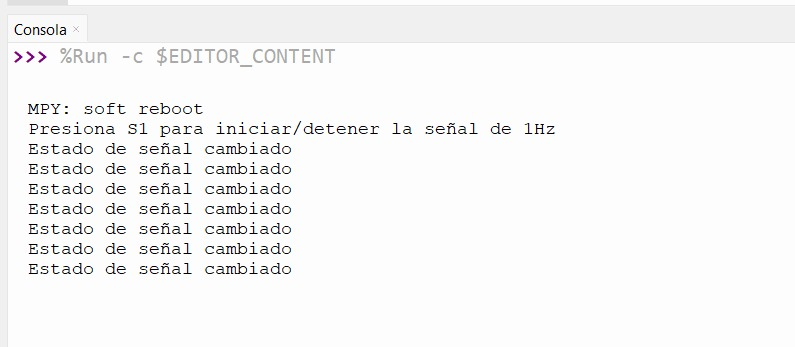
\includegraphics[width=0.85\textwidth]{img/Actividad2/Act2_3.jpg}
    \caption{Salida en consola mostrando los mensajes cada vez que se presiona S1 para alternar el estado de la se\~nal.}
\end{figure}

\subsection*{An\'alisis de resultados}

El programa logra alternar correctamente la generaci\'on de una se\~nal cuadrada de 1 Hz en el GPIO 20 cada vez que se presiona el bot\'on S1 conectado al GPIO 12. La variable global \texttt{generar\_senal} act\'ua eficazmente como mecanismo de comunicaci\'on entre la ISR (que se ejecuta en contexto de interrupci\'on) y el bucle principal. Al presionar S1 por primera vez, la bandera cambia a \texttt{True} y el LED comienza a parpadear con una frecuencia de 1 Hz (0.5 segundos encendido, 0.5 segundos apagado). Una segunda presi\'on desactiva la se\~nal, apagando el LED y deteniendo el parpadeo.
La implementaci\'on demuestra c\'omo las interrupciones permiten controlar procesos en tiempo real sin necesidad de sondeo constante, liberando la CPU para otras tareas mientras espera eventos externos.


    \section*{Actividad 3}
    \noindent Realizar un programa en el que se activen dos interrupciones, controladas por las
    entradas S1 y S2; en el momento de alguna de estas interrupciones sea requerida, genere las acciones
    solicitadas en la tabla 11-2.

    \begin{table}[h]
        \centering
        {\small
        \setlength{\tabcolsep}{3pt}
        \renewcommand{\arraystretch}{1.1}
        \arrayrulecolor{borderBlueB}
        \begin{tabular}{|l|l|l|l|}
            \hline
            \rowcolor{headerBlueB}
            \multicolumn{2}{|c|}{\textcolor{white}{\textbf{Evento}}} & \multicolumn{2}{c|}{\textcolor{white}{\textbf{Acciones}}} \\
            \hline
            \rowcolor{rowBlueB}
            \textbf{S1 (GPIO12)} & Pulso de bajada & LED ON (GPIO18) & TM1637 (GP0) Cuenta Interrupciones S1 \\
            \hline
            \rowcolor{white}
            \textbf{S2 (GPIO13)} & Pulso de bajada & LED ON (GPIO19) & TM1637 (GP10) Cuenta Interrupciones S2 \\
            \hline
        \end{tabular}
        }
        \vspace{0.3cm}
        \caption*{Tabla 11-2. Control; actividad 3}
    \end{table}

    \section*{Propuesta de solución}

    La solución propuesta para esta actividad consiste en configurar dos interrupciones externas por flanco de bajada, una para cada botón (S1 en GPIO12 y S2 en GPIO13), de manera que cada vez que se presione un botón se ejecute su respectiva rutina de servicio de interrupción (ISR). Dentro de cada ISR se enciende momentáneamente el LED asociado (GPIO18 para S1 y GPIO19 para S2), se incrementa un contador independiente y se actualiza el valor en su display TM1637 correspondiente (GP0/GP1 para S1 y GP10/GP11 para S2). Para evitar múltiples activaciones por rebote mecánico del botón, se incorpora un retardo de 300 ms dentro de cada ISR antes de apagar el LED. El programa principal permanece en un bucle infinito vacío, delegando toda la lógica de respuesta a las interrupciones de hardware.

    \begin{center}
    \scalebox{0.82}{
    \begin{tikzpicture}[node distance=1.1cm,
        startstop/.style={rectangle, rounded corners, minimum width=2.8cm, minimum height=0.7cm, align=center, draw=black, fill=red!30, font=\footnotesize},
        process/.style={rectangle, minimum width=3.2cm, minimum height=0.7cm, align=center, draw=black, fill=orange!30, font=\footnotesize},
        decision/.style={diamond, minimum width=2.5cm, minimum height=0.7cm, align=center, draw=black, fill=green!30, font=\footnotesize, aspect=2.5},
        io/.style={trapezium, trapezium left angle=70, trapezium right angle=110, minimum width=2.5cm, minimum height=0.7cm, align=center, draw=black, fill=blue!30, font=\footnotesize},
        arrow/.style={thick,->,>=stealth}]

        % Columna central - Programa principal
        \node (start) [startstop] {Inicio};
        \node (conf) [process, below=of start] {Configurar S1, S2\\como entrada PULL\_UP};
        \node (confleds) [process, below=of conf] {Configurar LED1 (GP18)\\LED2 (GP19) como salida};
        \node (conftm) [process, below=of confleds] {Inicializar displays\\TM1637 en 0};
        \node (irqconf) [process, below=of conftm] {Configurar IRQ\\S1 y S2 flanco bajada};
        \node (loop) [decision, below=of irqconf] {Bucle infinito\\(espera interrupciones)};
        \draw [arrow] (start) -- (conf);
        \draw [arrow] (conf) -- (confleds);
        \draw [arrow] (confleds) -- (conftm);
        \draw [arrow] (conftm) -- (irqconf);
        \draw [arrow] (irqconf) -- (loop);
        \draw [arrow] (loop.east) -- ++(0.8,0) |- (loop.north east);

        % Columna izquierda - ISR S1
        \node (isrs1) [startstop, left=3.5cm of conf] {ISR\_S1};
        \node (led1on) [process, below=of isrs1] {LED1 ON};
        \node (inc1) [process, below=of led1on] {contador\_s1 += 1};
        \node (disp1) [io, below=of inc1] {Mostrar contador\_s1\\en TM1637 (GP0)};
        \node (delay1) [process, below=of disp1] {Retardo 300 ms};
        \node (led1off) [process, below=of delay1] {LED1 OFF};
        \node (ret1) [startstop, below=of led1off] {Retorno};
        \draw [arrow] (isrs1) -- (led1on);
        \draw [arrow] (led1on) -- (inc1);
        \draw [arrow] (inc1) -- (disp1);
        \draw [arrow] (disp1) -- (delay1);
        \draw [arrow] (delay1) -- (led1off);
        \draw [arrow] (led1off) -- (ret1);

        % Columna derecha - ISR S2
        \node (isrs2) [startstop, right=3.5cm of conf] {ISR\_S2};
        \node (led2on) [process, below=of isrs2] {LED2 ON};
        \node (inc2) [process, below=of led2on] {contador\_s2 += 1};
        \node (disp2) [io, below=of inc2] {Mostrar contador\_s2\\en TM1637 (GP10)};
        \node (delay2) [process, below=of disp2] {Retardo 300 ms};
        \node (led2off) [process, below=of delay2] {LED2 OFF};
        \node (ret2) [startstop, below=of led2off] {Retorno};
        \draw [arrow] (isrs2) -- (led2on);
        \draw [arrow] (led2on) -- (inc2);
        \draw [arrow] (inc2) -- (disp2);
        \draw [arrow] (disp2) -- (delay2);
        \draw [arrow] (delay2) -- (led2off);
        \draw [arrow] (led2off) -- (ret2);

        % Flechas de interrupción
        \draw [arrow, dashed, red] (loop.west) -- ++(-1.2,0) node[midway, above, font=\tiny]{Interrupción S1} |- (isrs1.east);
        \draw [arrow, dashed, blue] (loop.east) -- ++(2.0,0) node[midway, above, font=\tiny]{Interrupción S2} |- (isrs2.west);

    \end{tikzpicture}
    }
    \end{center}

    En el diagrama de flujo se observan tres bloques: el programa principal (centro), que configura los pines de entrada con resistencia pull-up interna, los LEDs como salida, inicializa ambos displays TM1637 en cero y registra las interrupciones por flanco de bajada para S1 y S2; la ISR de S1 (izquierda), que al detectar la pulsación enciende el LED1, incrementa su contador, lo muestra en el display correspondiente, espera 300 ms como antirrebote y apaga el LED; y la ISR de S2 (derecha), que realiza el mismo procedimiento con el LED2 y su propio contador y display. El bucle principal permanece en espera pasiva, permitiendo que las interrupciones manejen toda la lógica de conteo y visualización.

    \section*{Desarrollo}

    \lstinputlisting[language={[LAB]Python}, caption=Código de la Actividad 3, basicstyle=\ttfamily\scriptsize]{Code/Act3.py}

    \begin{figure}[H]
        \centering
        
\includegraphics[width=0.75\textwidth]{img/Actividad3/Act3_1.jpg}
        \caption{Actividad 3: Estado inicial, primera pulsación de S2 con display S1 mostrando ``2'' y LED1 encendido.}
    \end{figure}

    \begin{figure}[H]
        \centering
        
\includegraphics[width=0.75\textwidth]{img/Actividad3/Act3_5.jpg}
        \caption{Actividad 3: Display S1 muestra ``12'' y display S2 muestra ``4'' tras múltiples pulsaciones.}
    \end{figure}

    \begin{figure}[H]
        \centering
        
\includegraphics[width=0.75\textwidth]{img/Actividad3/Act3_7.jpg}
        \caption{Actividad 3: Display S1 muestra ``5'' y display S2 en ``0'', LED1 encendido al presionar S1.}
    \end{figure}

    \begin{figure}[H]
        \centering
        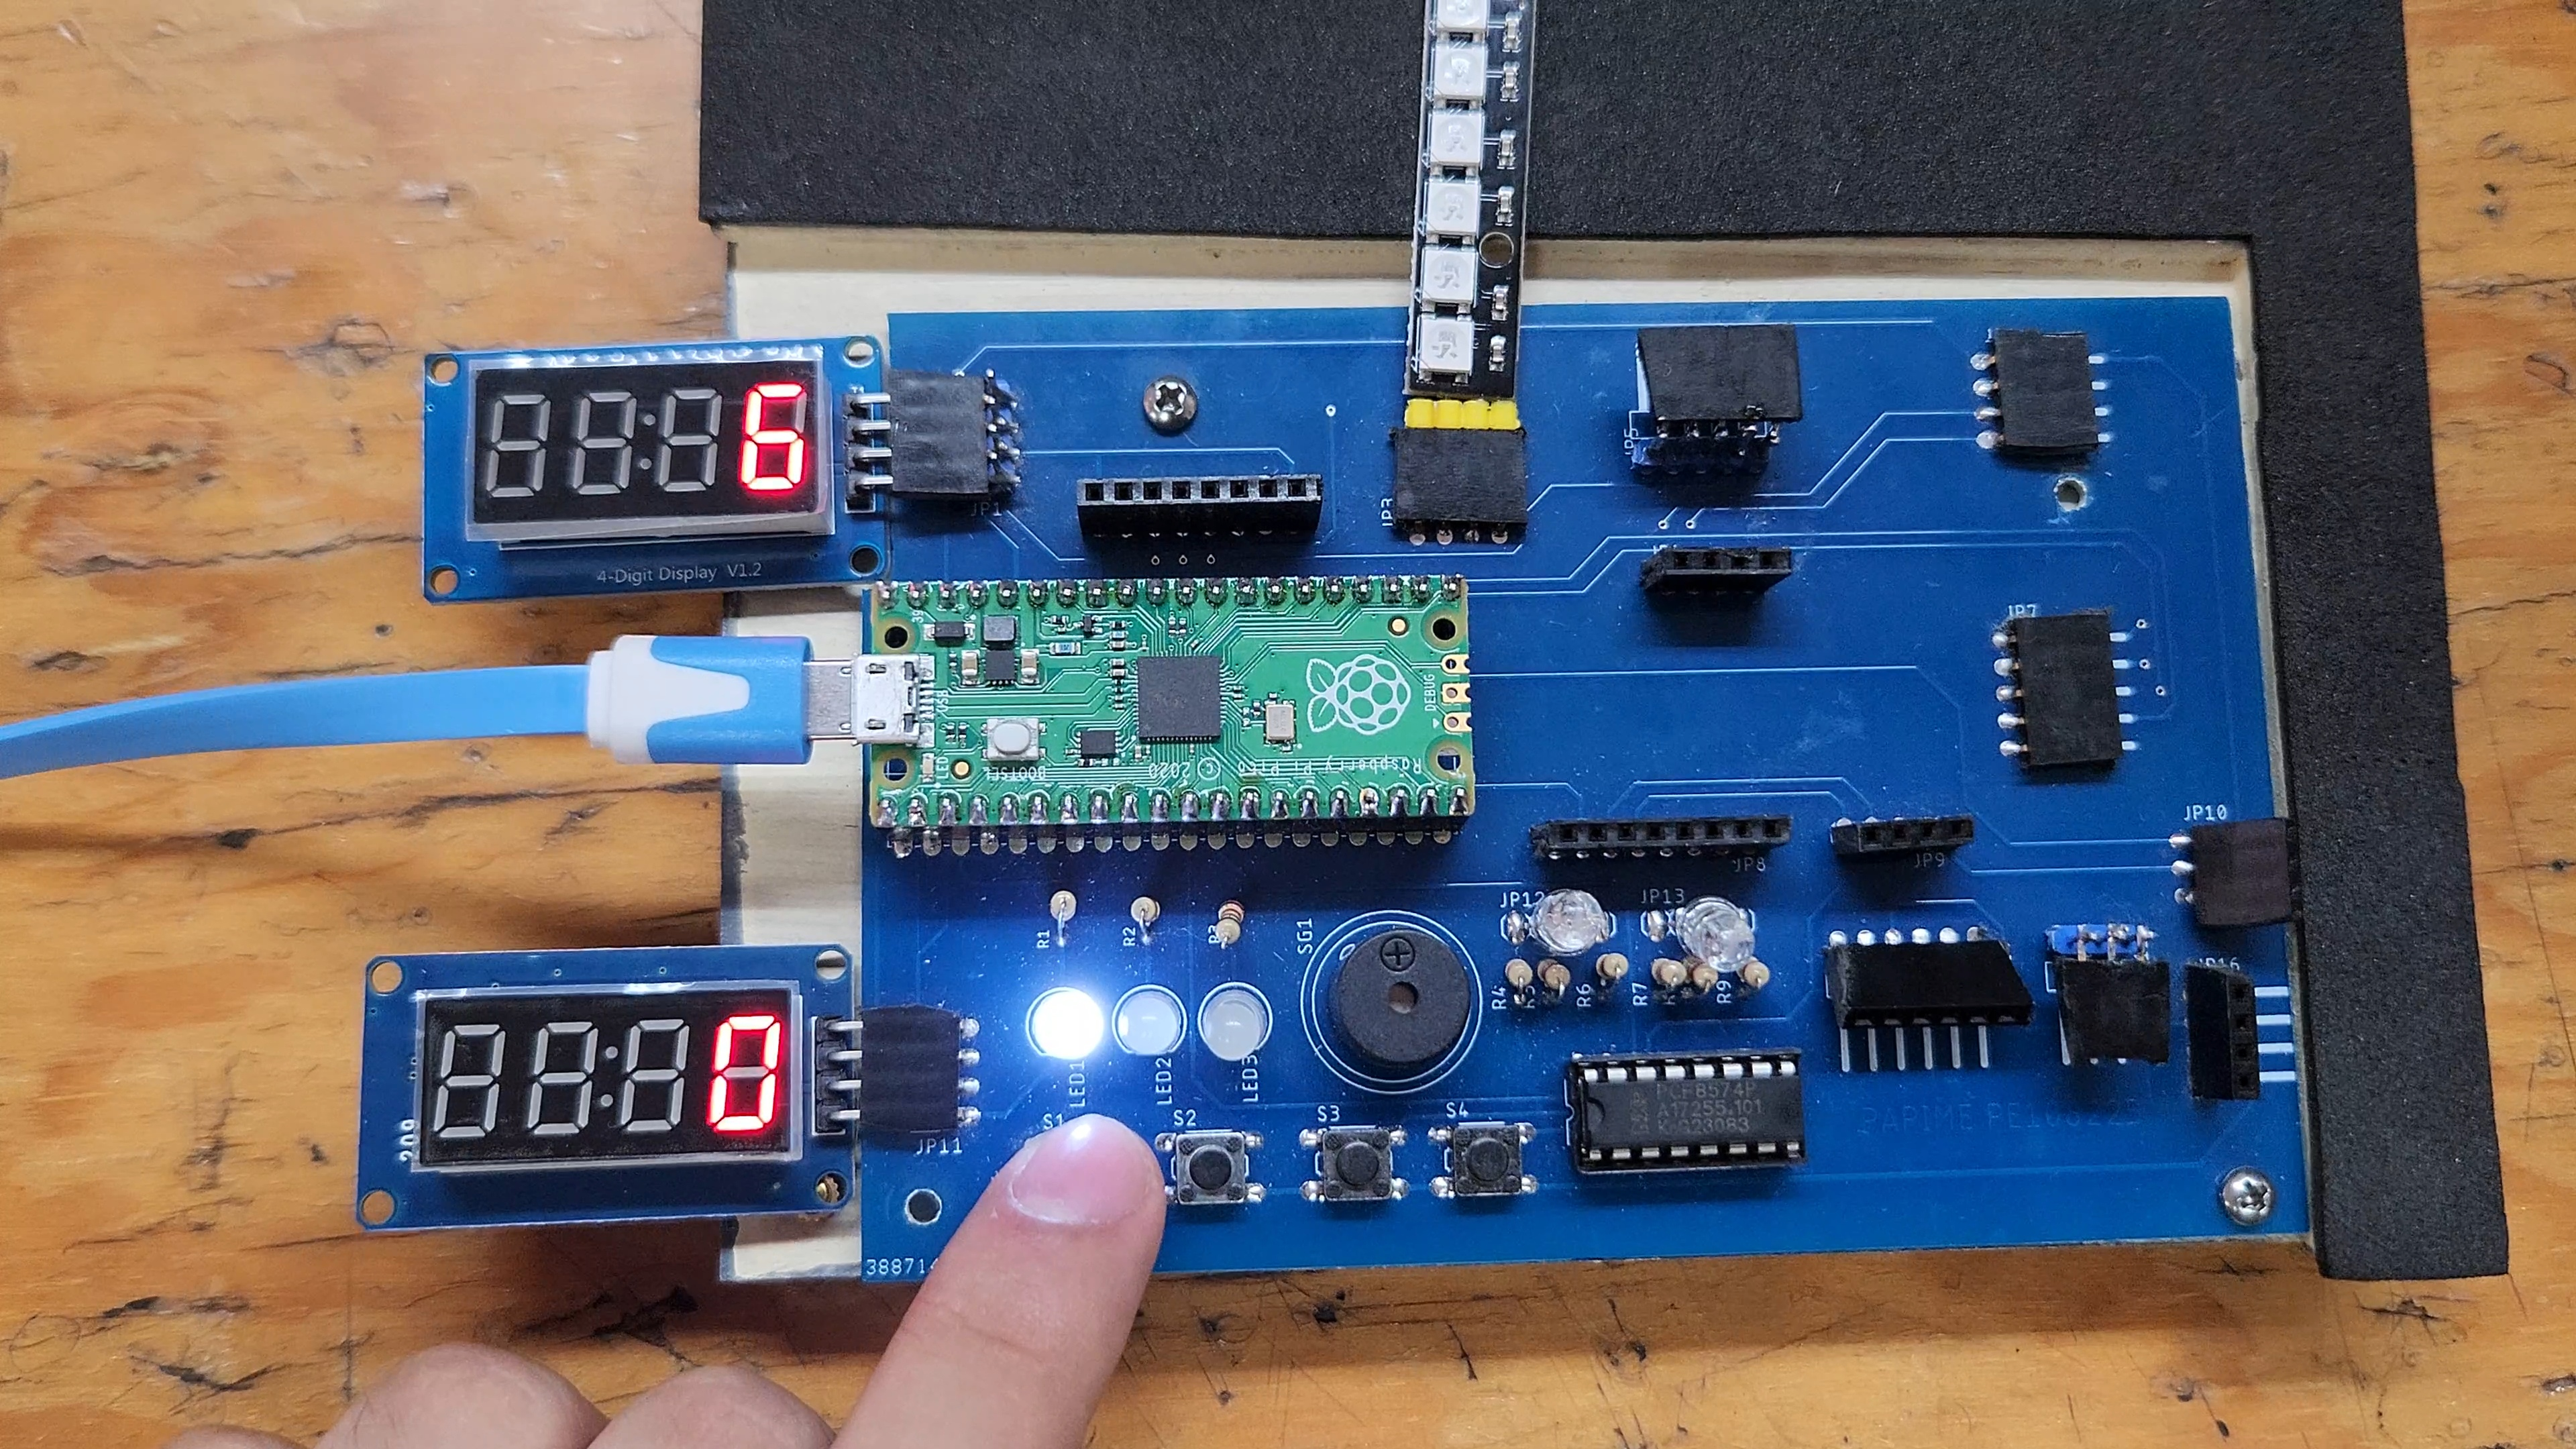
\includegraphics[width=0.75\textwidth]{img/Actividad3/Act3_8.jpg}
        \caption{Actividad 3: Display S1 muestra ``6'' y display S2 en ``0'', conteo ascendente de S1.}
    \end{figure}

    \begin{figure}[H]
        \centering
        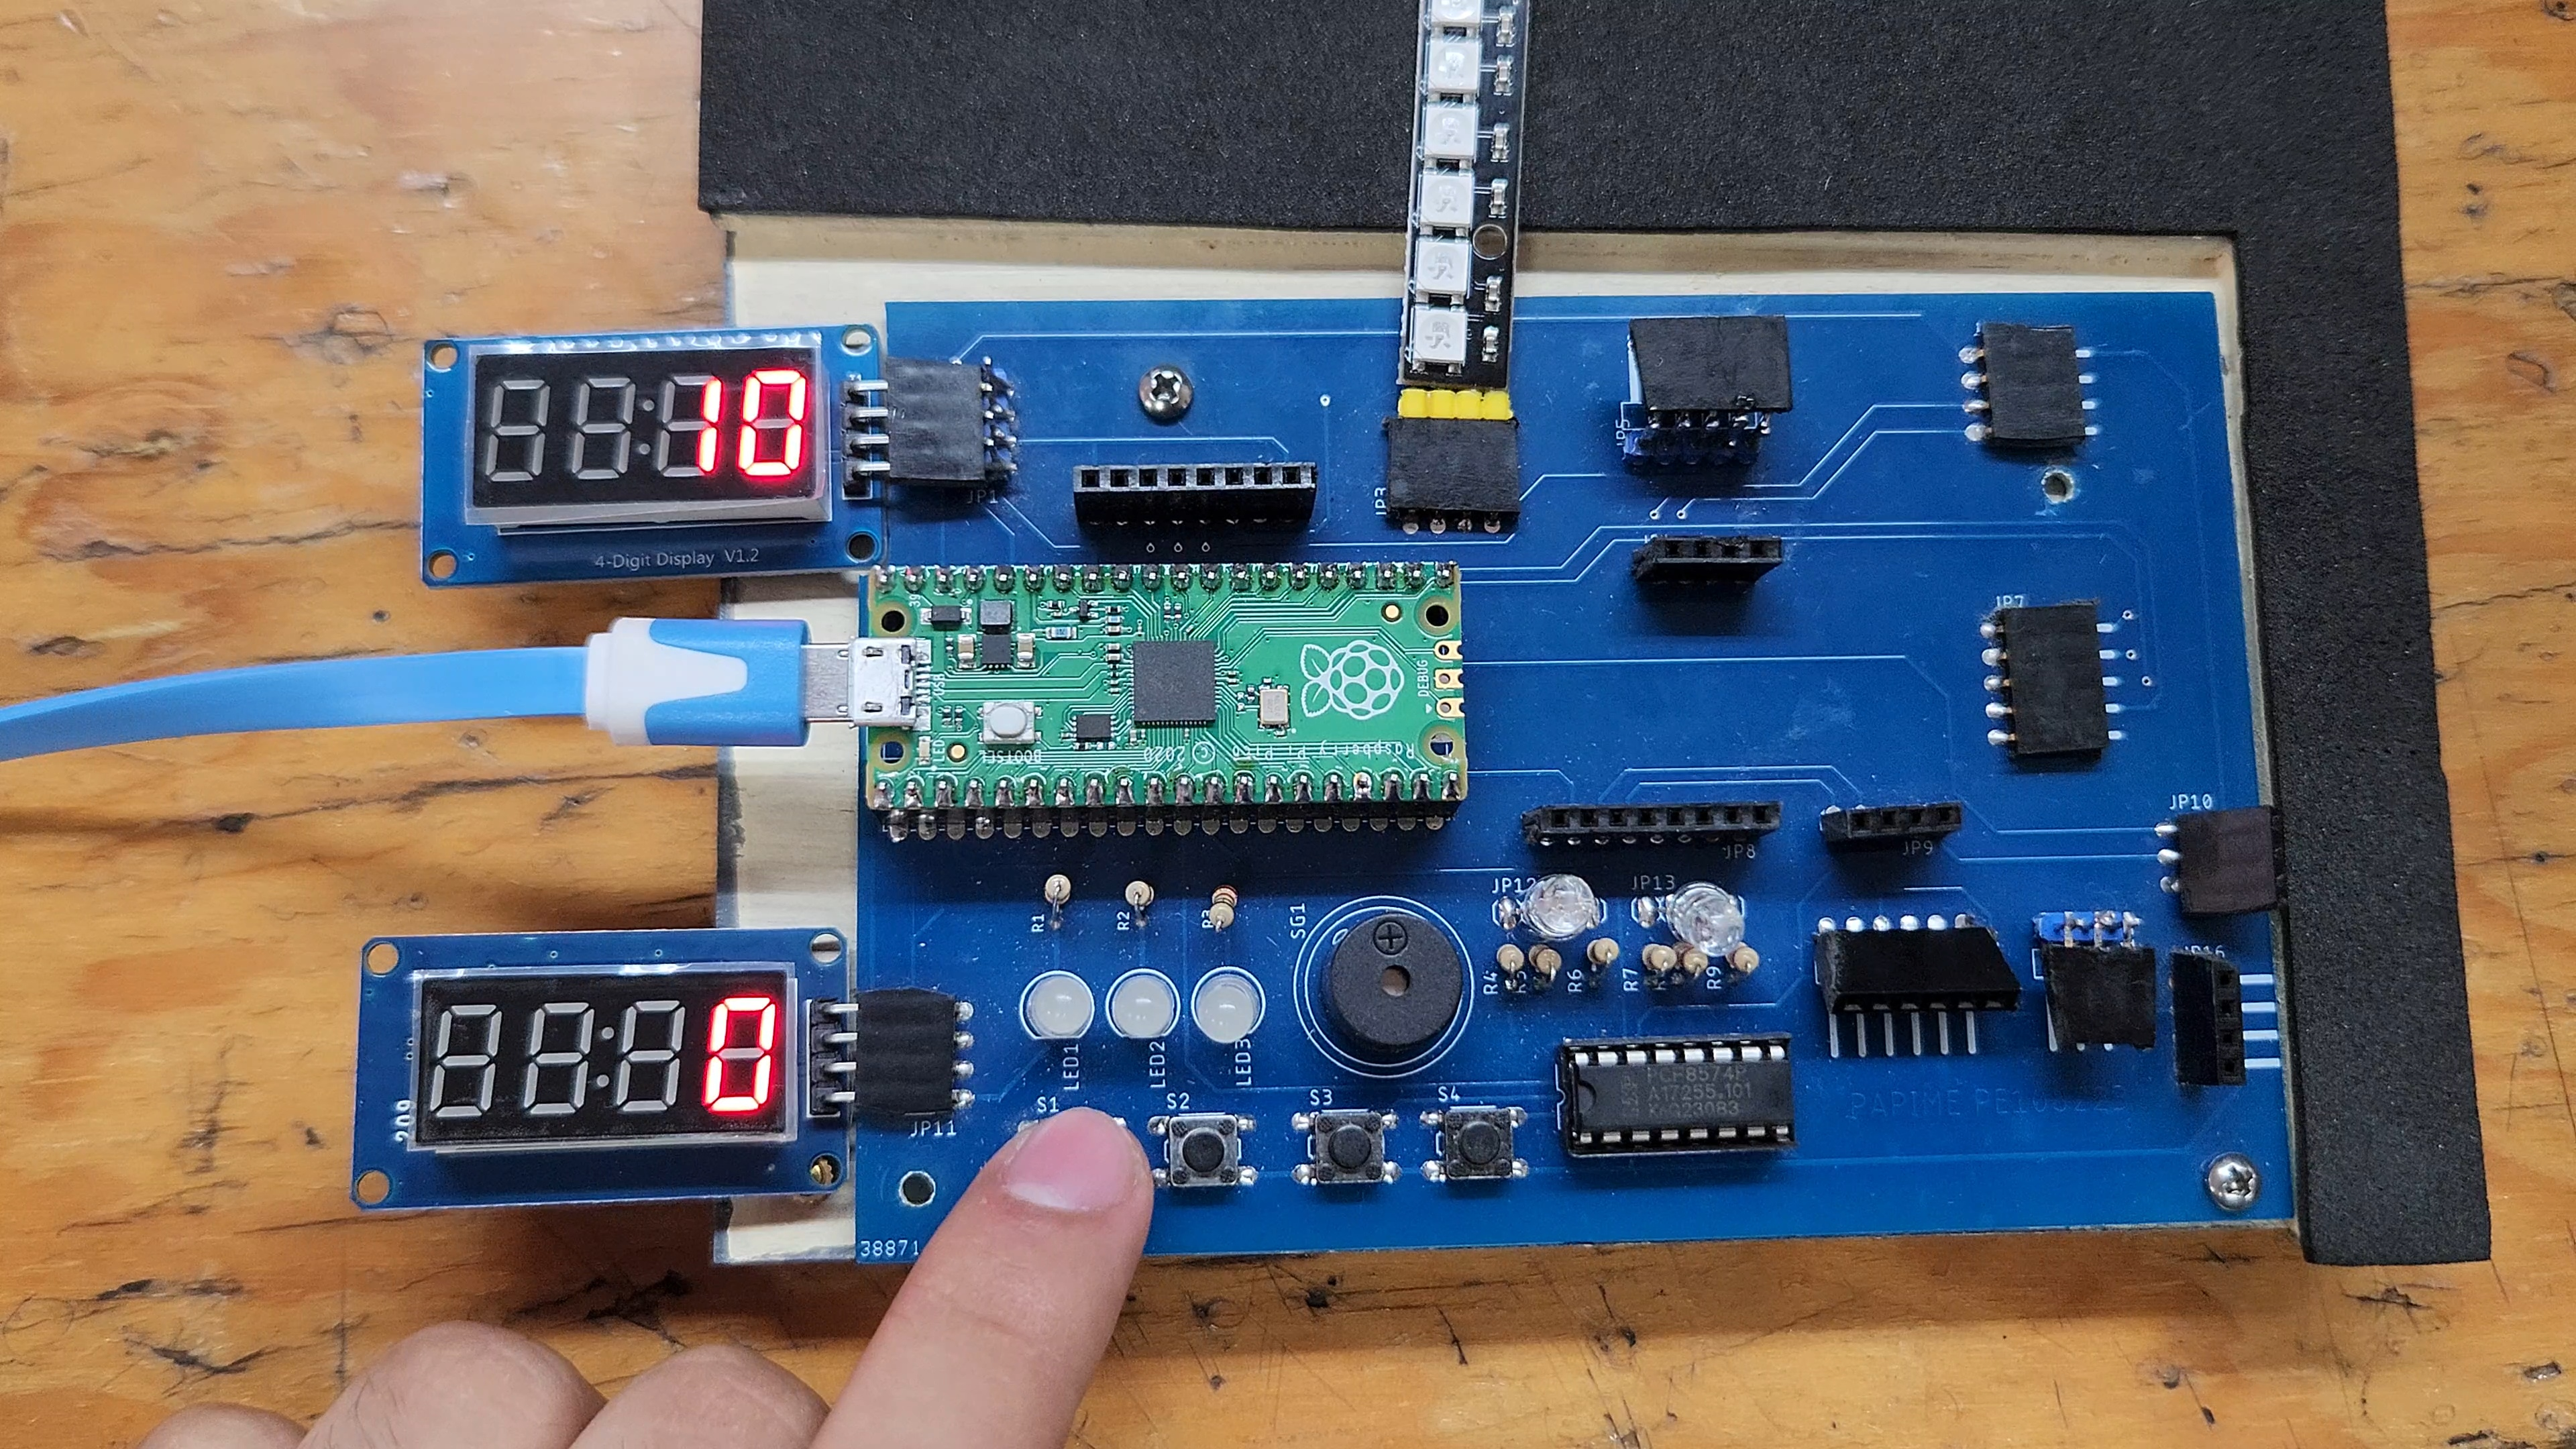
\includegraphics[width=0.75\textwidth]{img/Actividad3/Act3_12.jpg}
        \caption{Actividad 3: Display S1 muestra ``9'' y display S2 en ``0'', LED1 encendido tras pulsación.}
    \end{figure}

    \begin{figure}[H]
        \centering
        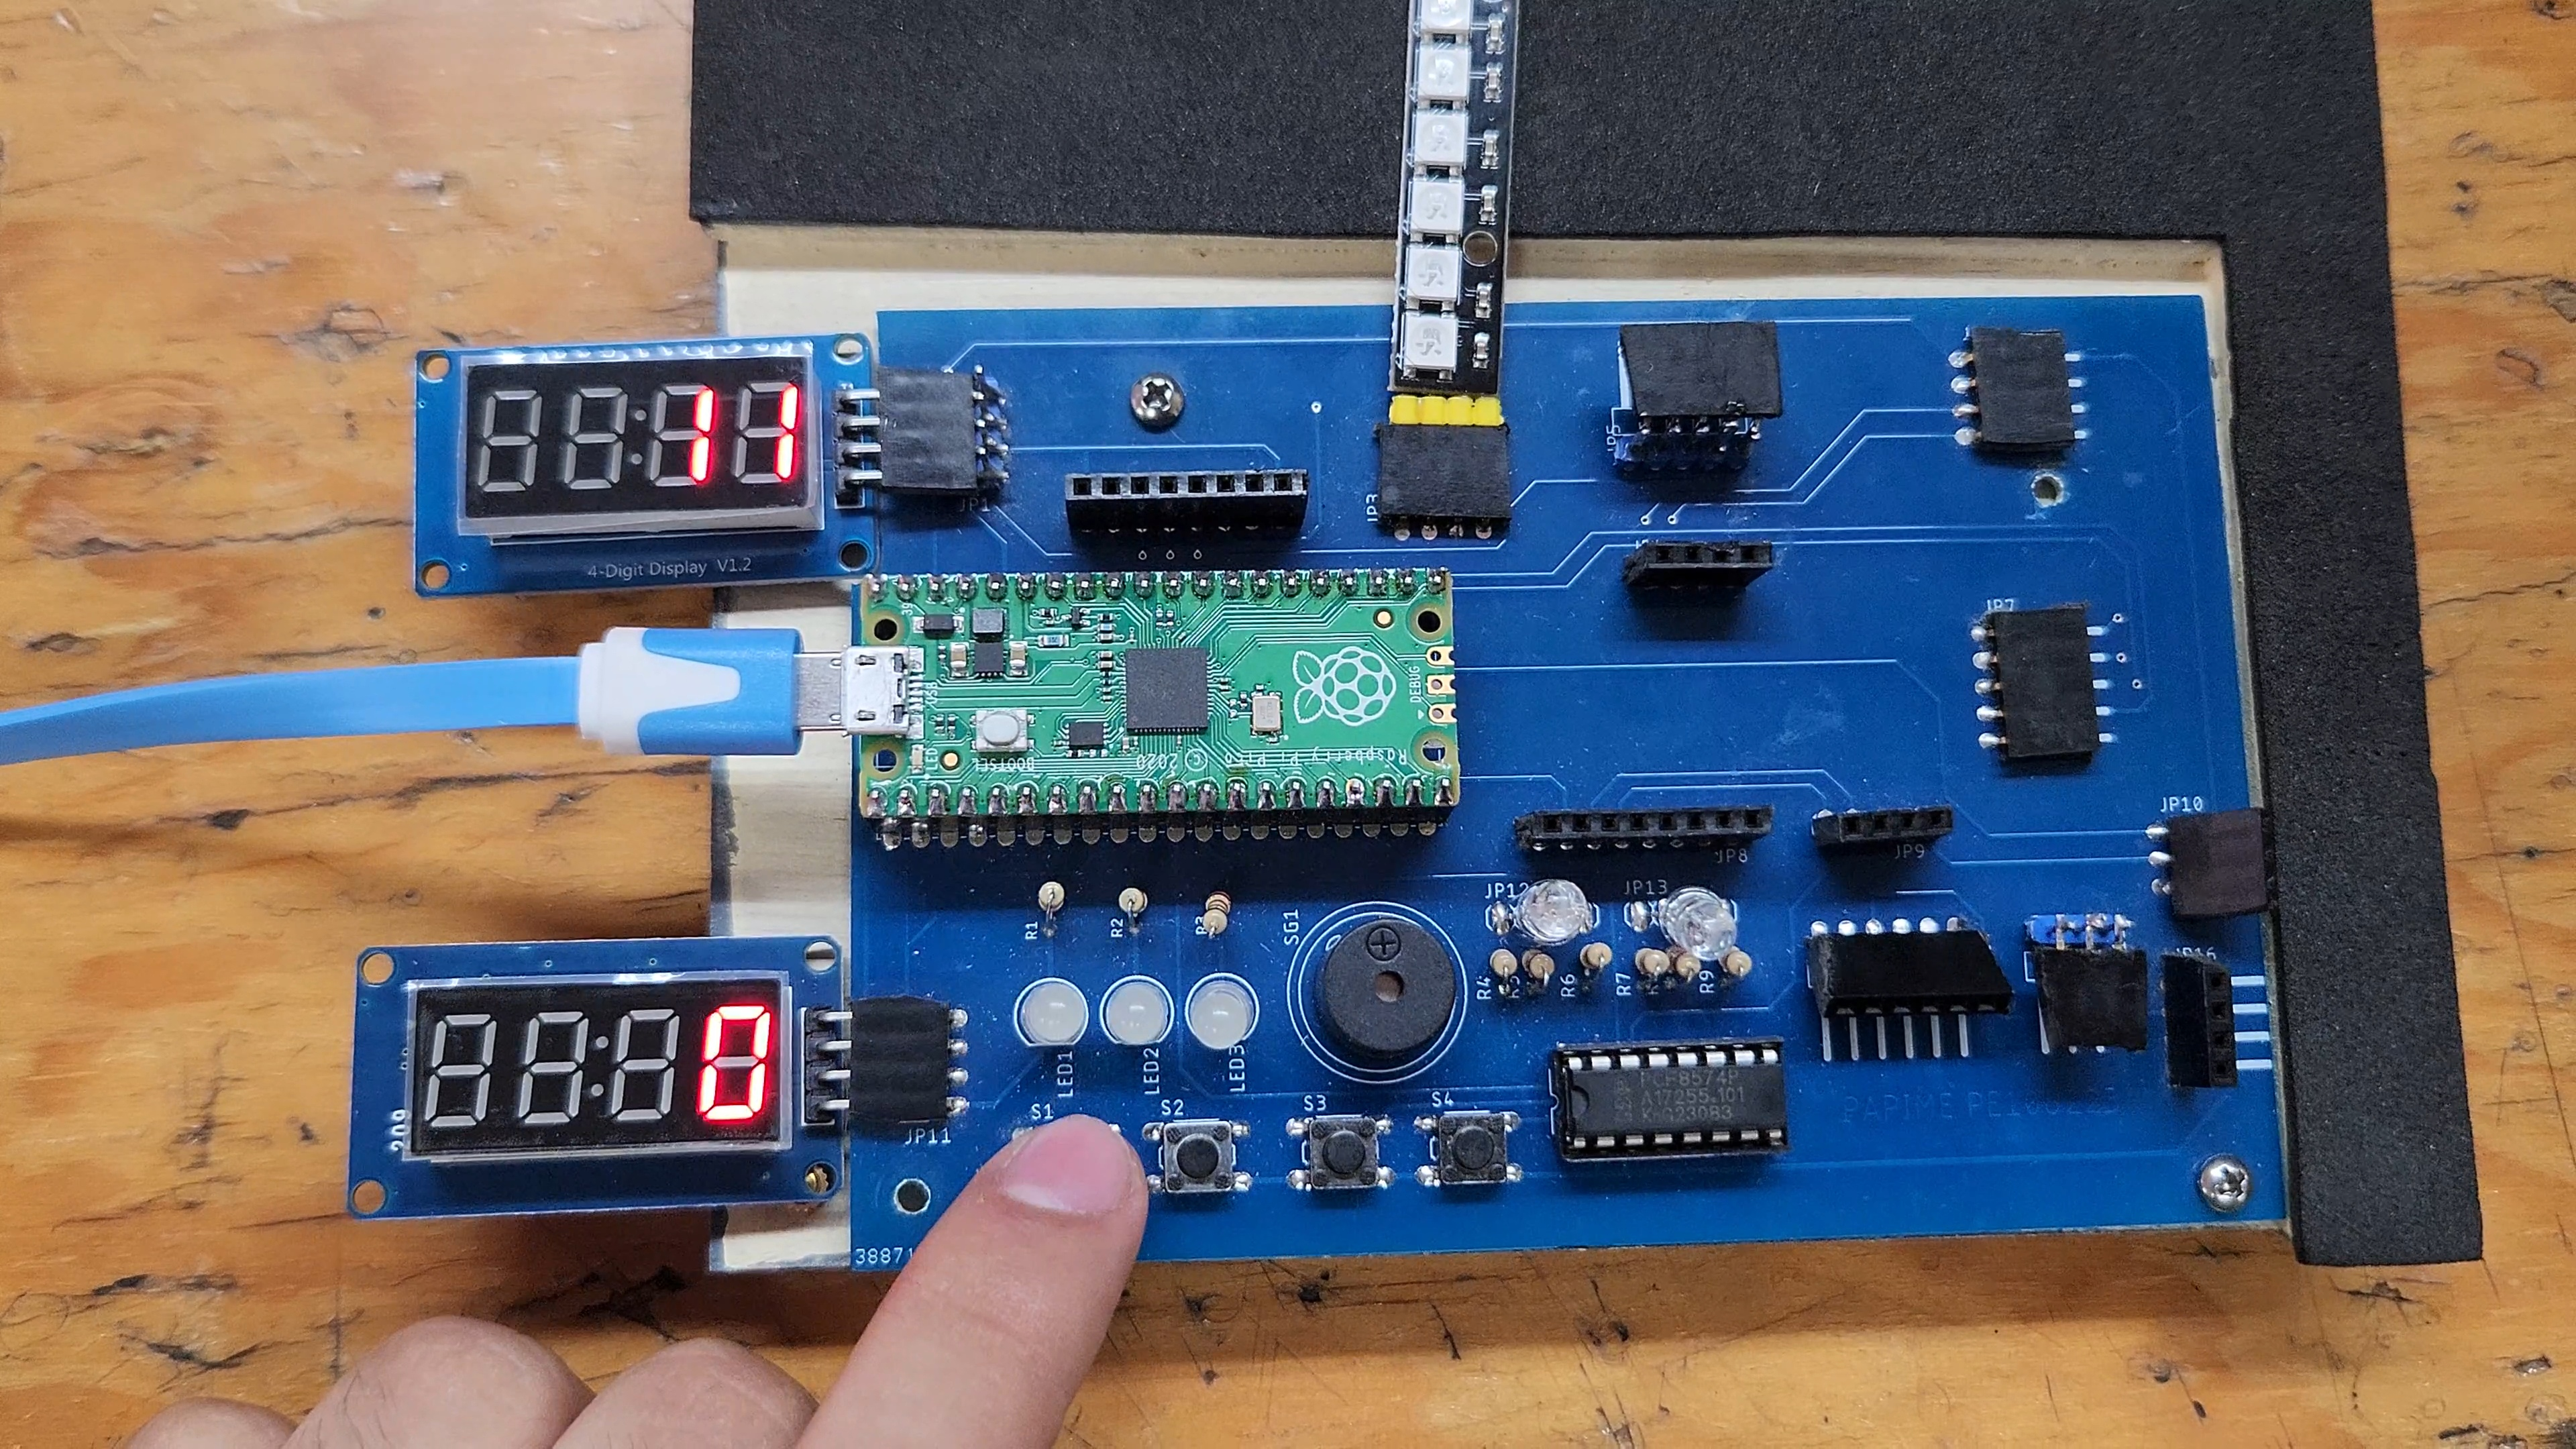
\includegraphics[width=0.75\textwidth]{img/Actividad3/Act3_13.jpg}
        \caption{Actividad 3: Display S1 alcanza ``10'' y display S2 permanece en ``0'', verificando conteo de dos dígitos.}
    \end{figure}

    \begin{figure}[H]
        \centering
        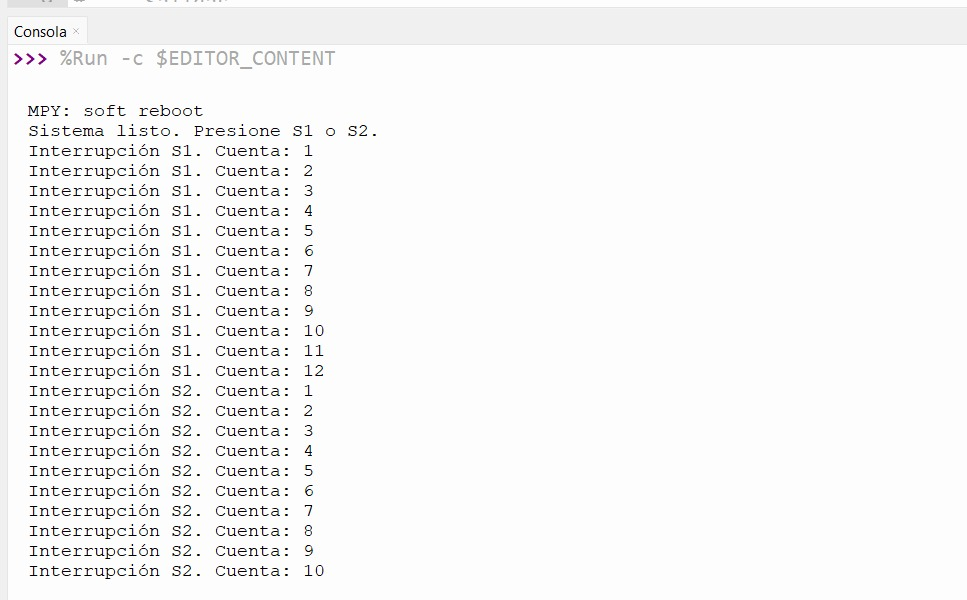
\includegraphics[width=0.75\textwidth]{img/Actividad3/Act3_15.jpg}
        \caption{Actividad 3: Salida en consola mostrando las interrupciones S1 (cuenta 1--12) y S2 (cuenta 1--10).}
    \end{figure}

    \subsection*{Análisis de resultados}

    Los resultados obtenidos en la Actividad 3 confirman el correcto funcionamiento del sistema de interrupciones externas implementado en la Raspberry Pi Pico. Como se observa en las Figuras 7 a 13, cada pulsación del botón S1 genera una interrupción por flanco de bajada que ejecuta la ISR correspondiente, incrementando el contador y actualizándolo en el display TM1637 conectado a los pines GP0 y GP1; de manera análoga, el botón S2 activa su propia ISR que actualiza el segundo display (GP10/GP11). En la Figura 7 se aprecia el estado tras la primera pulsación de S2 con el LED1 encendido y el display S1 mostrando el valor ``2'', lo cual demuestra que ambas interrupciones operan de forma independiente sin interferirse mutuamente. La Figura 8 evidencia que tras múltiples pulsaciones el display S1 alcanzó el valor 12 mientras que S2 llegó a 4, confirmando que los contadores son independientes y no se reinician entre pulsaciones. Las Figuras 9 a 12 muestran el conteo progresivo de S1 desde 5 hasta 9, verificando la consistencia del incremento unitario por cada pulsación y el encendido momentáneo del LED durante la ejecución de la ISR. La Figura 13 demuestra que el display TM1637 maneja correctamente valores de dos dígitos al mostrar ``10'', lo cual valida la función \texttt{tm\_s1.number()} de la librería. Finalmente, la Figura 14 muestra la salida en la consola serial, donde se imprime cada interrupción con su respectivo identificador (S1 o S2) y el valor acumulado del contador, alcanzando 12 pulsaciones para S1 y 10 para S2. El retardo de 300 ms implementado como antirrebote resultó efectivo, ya que no se observaron incrementos dobles o espurios en los contadores. La solución cumple con los objetivos planteados en la Tabla 11-2, demostrando el uso adecuado de interrupciones por hardware, la configuración de resistencias pull-up internas, la comunicación con periféricos TM1637 y el manejo de LEDs indicadores dentro de las rutinas de servicio de interrupción.

    \newpage

    \section*{Actividad 4}
    \noindent Escribir el siguiente código, comentar, indicar que hace y explicar su funcionamiento.

    \begin{lstlisting}[basicstyle=\ttfamily\footnotesize,caption={Figura 11-2. Código de ejemplo; actividad 1}]
    from machine import Pin
    import utime
    import _thread 

    led1 = Pin(18, Pin.OUT) 
    led2 = Pin(20, Pin.OUT) 

    def led2_thread():
        while True: 
            print("Este es un mensaje del segundo nucleo") 
            led2.toggle() 
            utime.sleep(0.2) 

    _thread.start_new_thread(led2_thread, ())

    while True: 
        led1.toggle() 
        utime.sleep(0.25) 
    \end{lstlisting}

    \section*{Propuesta de solución}


    En el código que se proporciona, lo primero que se realiza es la configuración de las bibliotecas necesarias, donde el módulo \texttt{machine} se utiliza para controlar los pines GPIO de la Raspberry Pi Pico, el módulo \texttt{utime} para manejar retardos y el módulo \texttt{\_thread} para crear hilos de ejecución en paralelo. 

    Ya con las bibliotecas importadas, se configuran dos pines como salida: el GPIO18 para controlar el LED1 y el GPIO20 para el LED2. Posteriormente en el programa se define una función llamada \texttt{led2\_thread()}, que contiene un bucle infinito donde se imprime un mensaje en la consola, se alterna el estado del LED2 y se introduce un retardo de 200 ms. Esta función es lanzada como un nuevo hilo de ejecución utilizando \texttt{\_thread.start\_new\_thread()}, lo que permite que el código dentro de esta función se ejecute concurrentemente con el resto del programa.

    Con la sentencia \texttt{\_thread.start\_new\_thread(led2\_thread, ())} se inicia el hilo que ejecutará la función \texttt{led2\_thread}, permitiendo que el mensaje y el parpadeo del LED2 ocurran de manera independiente al flujo principal del programa. Mientras tanto, el programa principal entra en un bucle infinito donde alterna el estado del LED1 cada 250 ms. Esto resulta en que ambos LEDs parpadeen a diferentes frecuencias (LED1 cada 250 ms y LED2 cada 200 ms) y que el mensaje del segundo núcleo se imprima continuamente en la consola sin bloquear la ejecución del programa principal.

    \begin{figure}[H]
        \centering
        \begin{tikzpicture}[node distance=1.1cm,
        startstop/.style={rectangle, rounded corners, minimum width=2.8cm, minimum height=0.7cm, align=center, draw=black, fill=red!30, font=\footnotesize},
        process/.style={rectangle, minimum width=3.2cm, minimum height=0.7cm, align=center, draw=black, fill=orange!30, font=\footnotesize},
        decision/.style={diamond, minimum width=2.5cm, minimum height=0.7cm, align=center, draw=black, fill=green!30, font=\footnotesize, aspect=2.5},
        io/.style={trapezium, trapezium left angle=70, trapezium right angle=110, minimum width=2.5cm, minimum height=0.7cm, align=center, draw=black, fill=blue!30, font=\footnotesize},
        arrow/.style={thick,->,>=stealth}]

        % Columna Izquierda - Hilo Principal (Core 0)
        \node (start0) [startstop] {Inicio (Main)};
        \node (init) [process, below=of start0] {Configurar LED1 (GP18)\\LED2 (GP20) como salida};
        \node (startthread) [process, below=of init] {Iniciar hilo secundario\\(led2\_thread)};
        \node (loop0) [decision, below=of startthread] {Bucle infinito\\(Core 0)};
        \node (toggle1) [process, below=of loop0] {Cambiar estado\\LED1 (toggle)};
        \node (sleep1) [process, below=of toggle1] {Retardo 250 ms};

        % Conexiones Hilo Principal
        \draw [arrow] (start0) -- (init);
        \draw [arrow] (init) -- (startthread);
        \draw [arrow] (startthread) -- (loop0);
        \draw [arrow] (loop0) -- (toggle1);
        \draw [arrow] (toggle1) -- (sleep1);
        % Retorno del bucle principal
        \draw [arrow] (sleep1.west) -- ++(-1.2,0) |- (loop0.west);


        % Columna Derecha - Segundo Hilo (Core 1)
        \node (start1) [startstop, right=3.5cm of startthread] {Inicio Hilo\\(led2\_thread)};
        \node (loop1) [decision, below=of start1] {Bucle infinito\\(Core 1)};
        \node (print) [io, below=of loop1] {Este es un mensaje del \\ segundo nucleo};
        \node (toggle2) [process, below=of print] {Cambiar estado\\LED2 (toggle)};
        \node (sleep2) [process, below=of toggle2] {Retardo 200 ms};

        % Conexiones Segundo Hilo
        \draw [arrow] (start1) -- (loop1);
        \draw [arrow] (loop1) -- (print);
        \draw [arrow] (print) -- (toggle2);
        \draw [arrow] (toggle2) -- (sleep2);
        % Retorno del bucle secundario
        \draw [arrow] (sleep2.east) -- ++(1.2,0) |- (loop1.east);

        % Flecha indicadora de creación de hilo (Lógica concurrente)
        \draw [arrow, dashed, blue] (startthread.east) -- node[midway, above, font=\tiny]{\_thread.start\_new\_thread} (start1.west);

        \end{tikzpicture}
    \end{figure}

    \section*{Desarrollo}

    \lstinputlisting[language={[LAB]Python}, caption=Código de la Actividad 4, basicstyle=\ttfamily\scriptsize]{Code/Act4.py}

    
    \begin{figure}[H]
        \centering
        
\includegraphics[width=0.75\textwidth]{img/Actividad4/Act4_3.jpg}
        \caption{Ambos LEDS apagados.}
    \end{figure}

    \begin{figure}[H]
        \centering
        
\includegraphics[width=0.75\textwidth]{img/Actividad4/Act4_4.jpg}
        \caption{Ambos LEDS encendidos.}
    \end{figure}


    \begin{figure}[H]
        \centering
        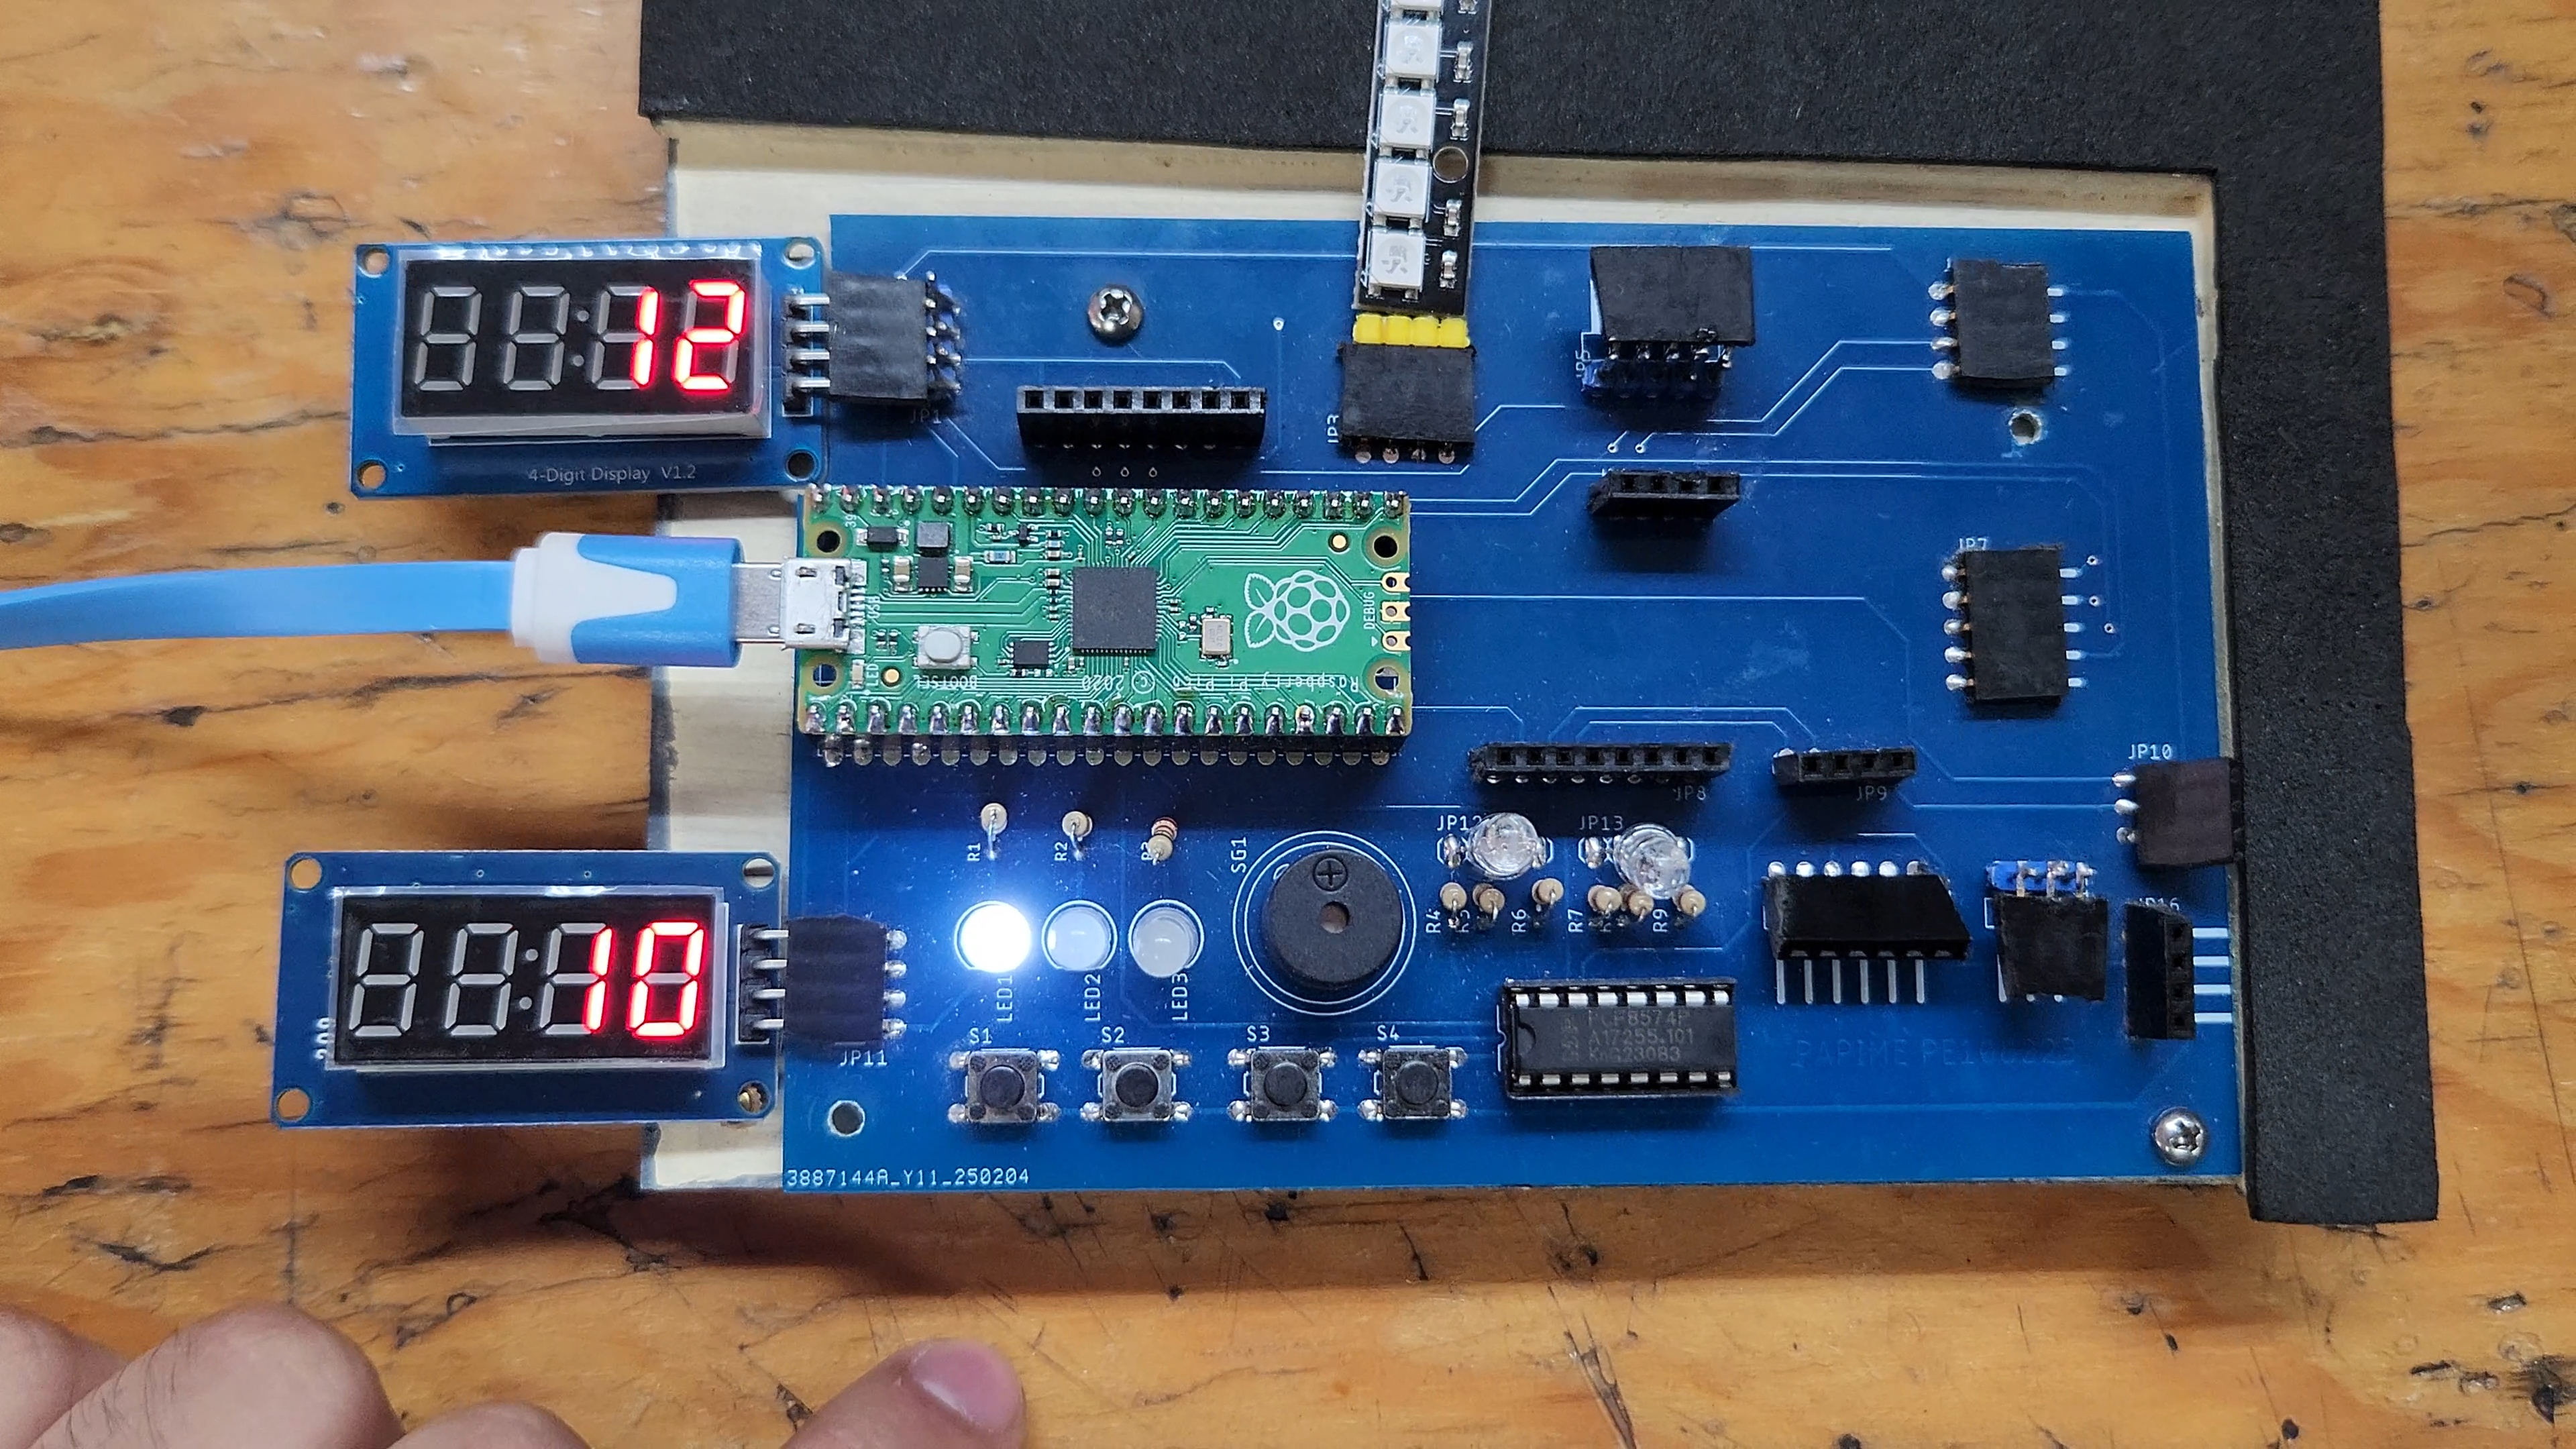
\includegraphics[width=0.75\textwidth]{img/Actividad4/Act4_5.jpg}
        \caption{Led 1 encendido, Led 2 apagado}
    \end{figure}

    \begin{figure}[H]
        \centering
        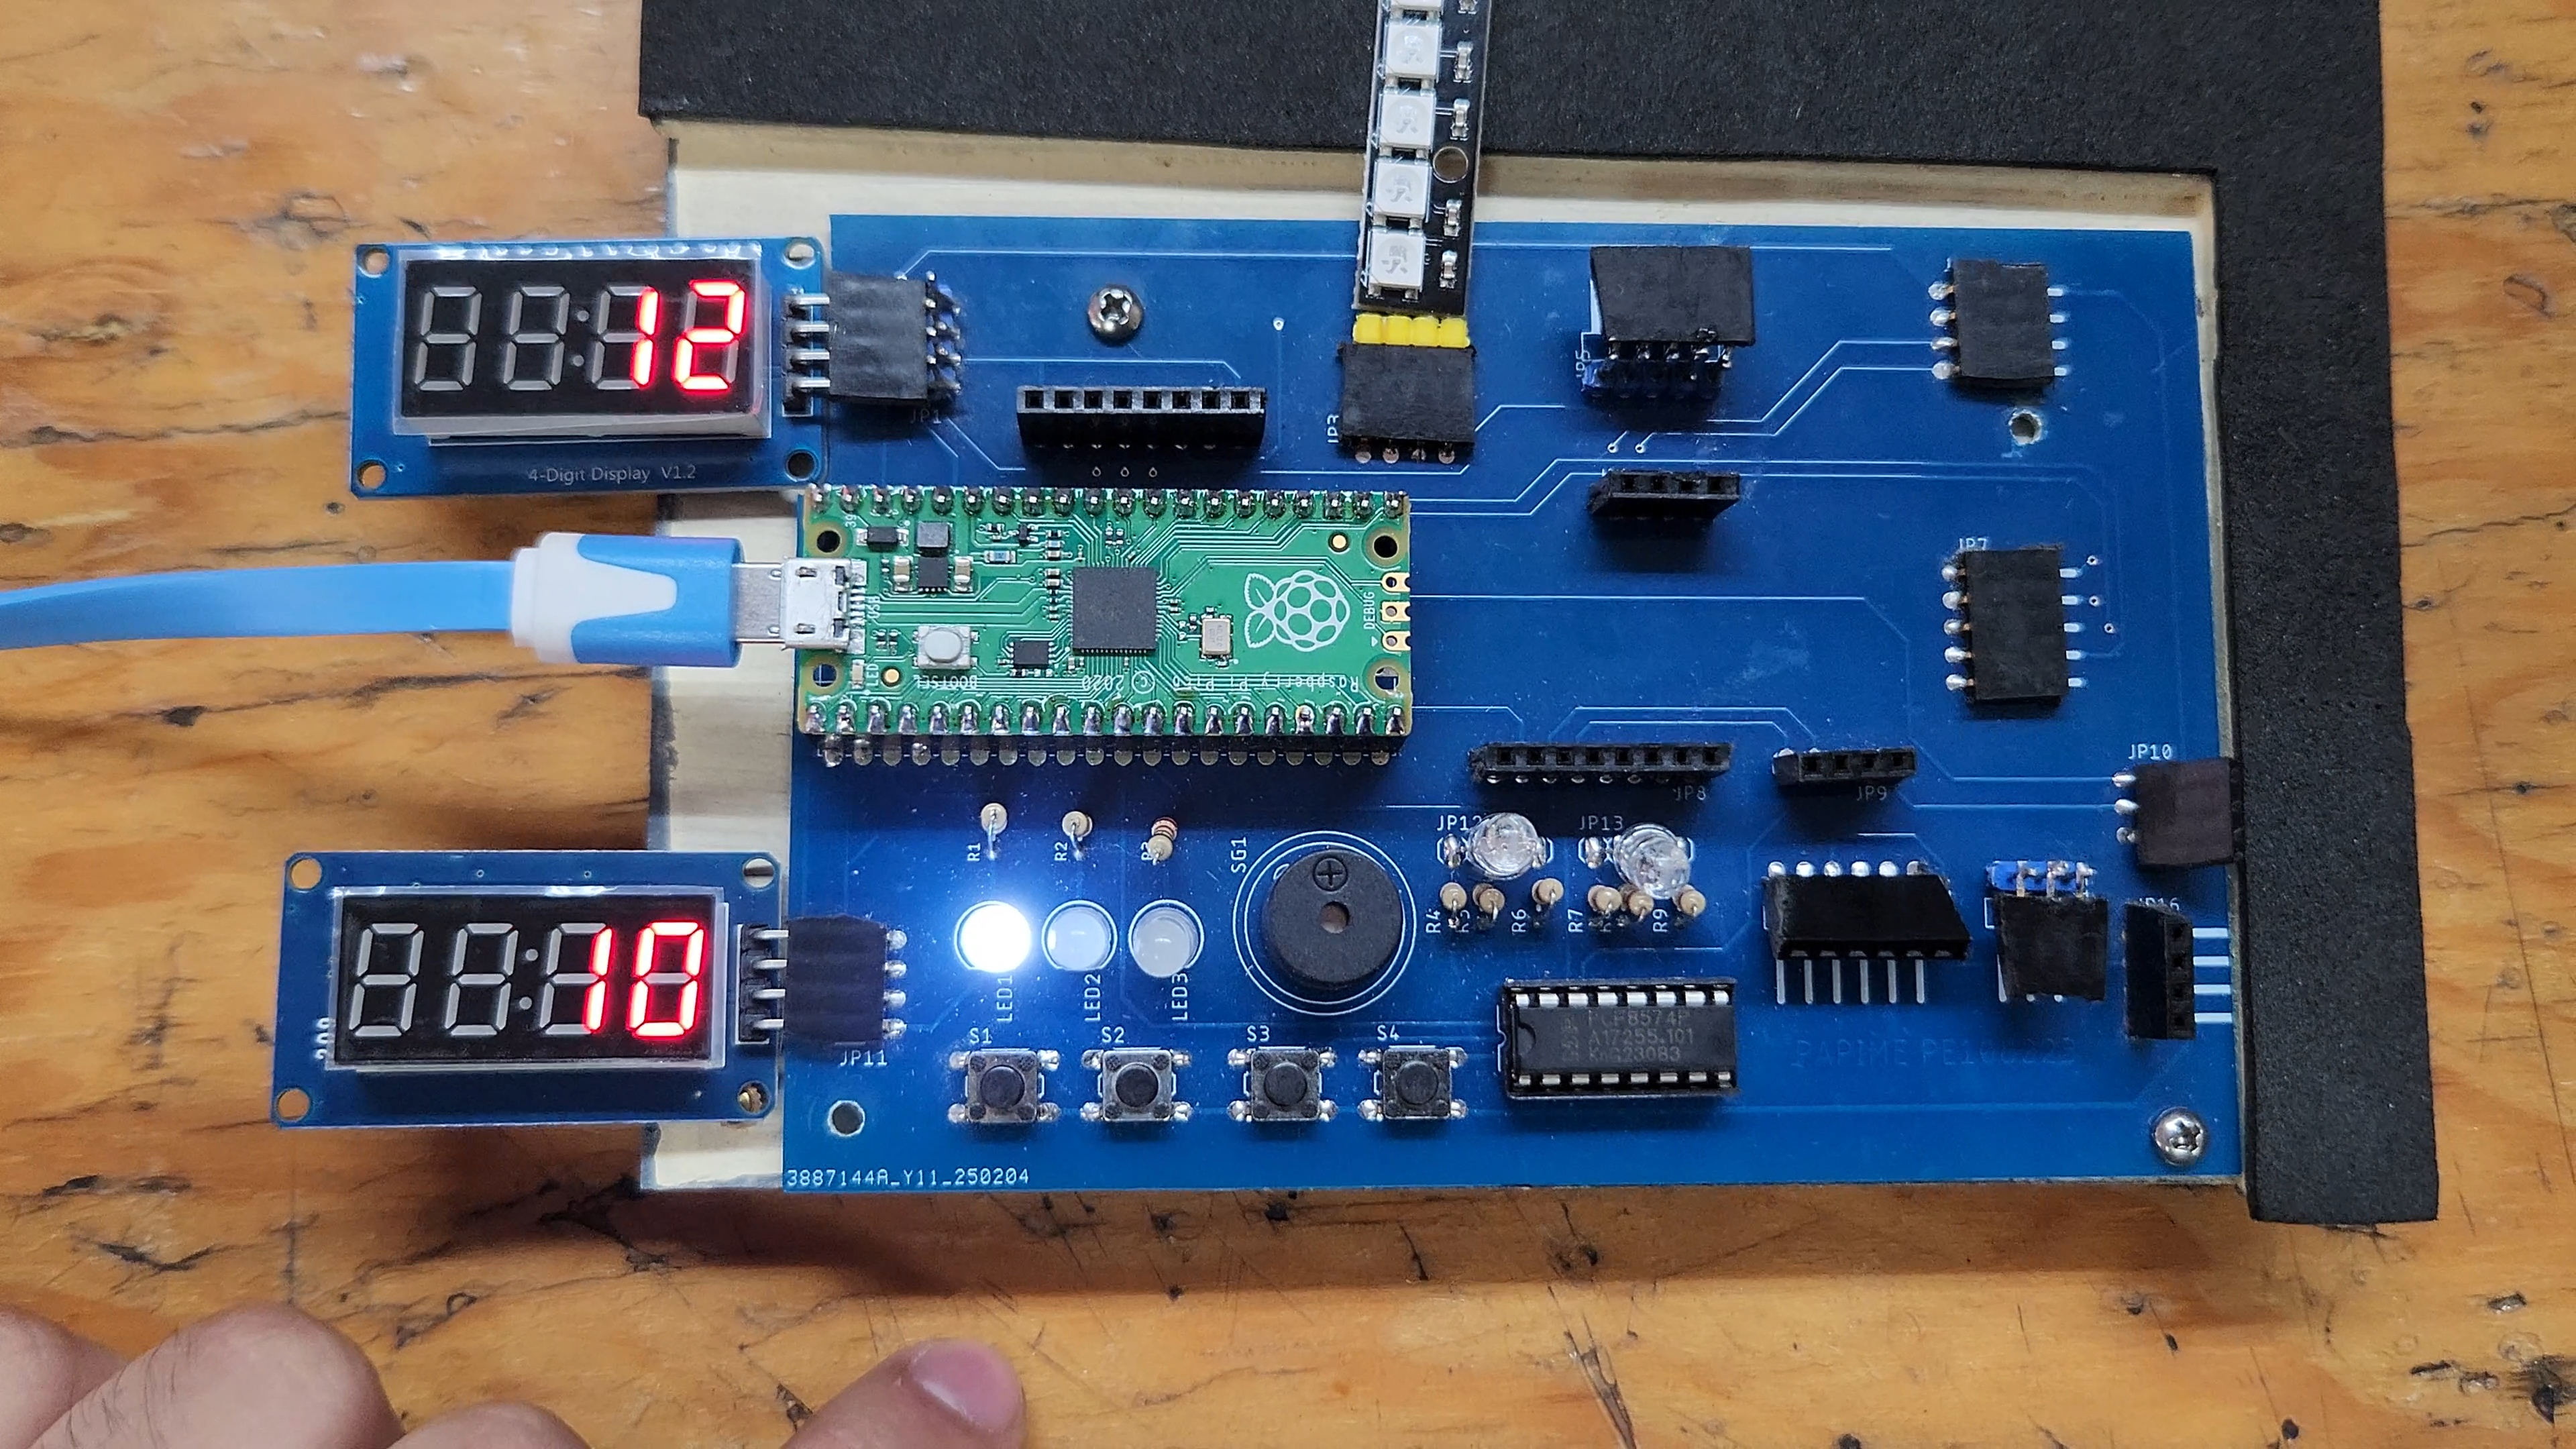
\includegraphics[width=0.75\textwidth]{img/Actividad4/Act4_5.jpg}
        \caption{Mensajes del segundo núcleo visibles en la consola}
    \end{figure}

    \subsection*{Análisis de resultados}

    A partir de las imagenes obtenidas en la Actividad 4, se puede concluir que el programa implementa correctamente la ejecución concurrente utilizando hilos en la Raspberry Pi Pico. En las Figuras se observa el estado inicial del sistema, donde ambos LEDs (LED1 en GPIO18 y LED2 en GPIO20) están apagados, lo cual es consistente con la configuración inicial del programa. En la siguiente figura se muestran ambos LEDs encendidos simultáneamente, lo que indica que el hilo principal (Core 0) y el hilo secundario (Core 1) están ejecutándose correctamente y alternando el estado de sus respectivos LEDs. En la tercera figura se muestra el LED1 encendido mientras el LED2 está apagado, lo que confirma que cada hilo controla su propio LED de manera independiente sin interferencias. Finalmente, en la última figura se pueden observar los mensajes impresos por el segundo núcleo en la consola, lo que demuestra que el hilo secundario está activo y ejecutando su función de impresión y parpadeo del LED2. De forma que el programa muestra un comportamiento esperado de concurrencia, con ambos hilos operando de manera simultánea y sin bloqueos, validando el uso de la librería \texttt{\_thread} para la creación de hilos en la Raspberry Pi Pico.


    \newpage
    \section*{Actividad 5}
    \noindent Realizar un programa, que sea controlado con interrupciones, serán activadas cada que
    se detecten flancos de bajada en S1 y S2; cuando sean reconocidas generar las acciones solicitadas
    en la tabla 11-4; considerar que estas serán ejecutadas en diferentes núcleos.

    \begin{table}[h]
        \centering
        \renewcommand{\arraystretch}{1.2}
        \setlength{\arrayrulewidth}{1pt}
        \arrayrulecolor{white} % Bordes blancos para el estilo naranja
        \begin{tabular}{|c|c|c|c|c|}
            \hline
            \rowcolor{TabOrangeHead}
            \multicolumn{2}{|c|}{\textcolor{white}{\textbf{Evento}}} & \multicolumn{3}{c|}{\textcolor{white}{\textbf{Acción}}} \\
            \hline
            \rowcolor{TabOrangeHead}
            \textcolor{white}{\textbf{Interrupción}} & \textcolor{white}{\textbf{Hilo (Thread)}} & \textcolor{white}{\textbf{LED}} & \textcolor{white}{\textbf{Estado}} & \textcolor{white}{\textbf{Hilo (Thread)}} \\
            \hline
            \rowcolor{TabOrangeBody}
            \cellcolor{TabOrangeHead}\textcolor{white}{\textbf{S1}} & 1 & GPIO18 & Toggle & 1 \\
            \hline
            \rowcolor{TabOrangeBody}
            \cellcolor{TabOrangeHead}\textcolor{white}{\textbf{S2}} & 1 & GPIO19 & Toggle & 2 \\
            \hline
        \end{tabular}
        \vspace{0.3cm}
        \caption*{Tabla 11-4. Acciones de control; actividad 5}
    \end{table}

    \section*{Propuesta de solución}

    De acuerdo a los requerimientos de la Actividad 5, es necesario controlar los interruptores S1 y S2 mediante interrupciones externas por flanco de bajada, es por esto que primero se deben de realizar la importación de las bibliotecas necesarias para el manejo de pines, interrupciones y hilos. 
    
    Posteriormente se configuran los pines GPIO18 y GPIO19 como salidas para controlar los LEDs asociados a cada interruptor y como entradas con resistencia pull-up para los interruptores S1 (GPIO12) y S2 (GPIO13). Despúes se declara una bandera con la finalidad de comunicar el estado de la interrupción entre los hilos, y se inicializan dos contadores para llevar el registro de las interrupciones de cada botón.

    A continuación, se definen dos funciones para las rutinas de servicio de interrupción (ISR) de S1 y S2, donde para la rutina de interrupción que se ejecuta en el Núcleo 1 (Core 0) se maneja la interrupción de S1, encendiendo el LED en GPIO18 e imprimiendo un mensaje en la consola, mientras que para la rutina de interrupción que se ejecuta en el Núcleo 2 (Core 1) se maneja la interrupción de S2 modificando la bandera para indicar que se ha detectado la interrupción.

    En el programa se tiene la función \texttt{nucleo\_dos()} que se ejecuta en el segundo núcleo, donde se monitorea continuamente la bandera para detectar si se ha producido una interrupción en S2. Si la bandera indica que se ha detectado una interrupción, se enciende el LED en GPIO19, se imprime un mensaje en la consola y se restablece la bandera para esperar la siguiente interrupción.

    Por otro lado el bucle principal del programa se mantiene en espera pasiva, permitiendo que las interrupciones manejen toda la lógica de respuesta a los eventos de los botones. De esta manera, se logra que cada botón controle su propio LED y que las acciones asociadas a cada interrupción se ejecuten en diferentes núcleos, cumpliendo con los requerimientos establecidos en la Tabla.

    \begin{figure}[H]
        \centering
        \scalebox{0.62}{
        \begin{tikzpicture}[node distance=1.1cm and 0.6cm,
            startstop/.style={rectangle, rounded corners, minimum width=2.8cm, minimum height=0.7cm, align=center, draw=black, fill=red!30, font=\footnotesize},
            process/.style={rectangle, minimum width=3.2cm, minimum height=0.7cm, align=center, draw=black, fill=orange!30, font=\footnotesize},
            decision/.style={diamond, minimum width=2.5cm, minimum height=0.7cm, align=center, draw=black, fill=green!30, font=\footnotesize, aspect=2.5},
            io/.style={trapezium, trapezium left angle=70, trapezium right angle=110, minimum width=2.5cm, minimum height=0.7cm, align=center, draw=black, fill=blue!30, font=\footnotesize},
            arrow/.style={thick,->,>=stealth}]

            % --- Columna Central: Hilo Principal (Core 0) ---
            \node (start) [startstop] {Inicio (Main)};
            \node (conf) [process, below=of start] {Configurar Entradas/Salidas\\S1, S2, LED1, LED2};
            \node (flag) [process, below=of conf] {flag\_s2\_presionado = False};
            \node (thread) [process, below=of flag] {\_thread.start\_new\_thread\\(nucleo\_dos)};
            \node (irq) [process, below=of thread] {Configurar IRQ\\(S1 $\to$ isr\_s1, S2 $\to$ isr\_s2)};
            \node (printm) [io, below=of irq] {Multinucleo listo \\ Presione S1 o S2...};
            \node (loop0) [decision, below=of printm] {Bucle infinito\\(while True: pass)};

            \draw [arrow] (start) -- (conf);
            \draw [arrow] (conf) -- (flag);
            \draw [arrow] (flag) -- (thread);
            \draw [arrow] (thread) -- (irq);
            \draw [arrow] (irq) -- (printm);
            \draw [arrow] (printm) -- (loop0);
            \draw [arrow] (loop0.east) -- ++(0.8,0) |- (loop0.north east);

            % --- Columna Derecha: Hilo Secundario (Core 1) ---
            \node (start1) [startstop, right=3.5cm of conf] {Inicio Hilo\\(nucleo\_dos)};
            \node (loop1) [decision, below=of start1] {Bucle infinito};
            \node (check) [decision, below=of loop1] {¿flag\_s2\_presionado\\== True?};
            \node (act1) [process, right=0.4cm of check] {Toggle LED2\\flag\_s2\_presionado = False};
            \node (print2) [io, below=of act1] {Núcleo 2: Toggle LED 2};
            \node (act2) [process, below=of print2] {Retardo 300 ms};
            \node (sleep10) [process, below=of check] {Retardo 10 ms};

            \draw [arrow] (start1) -- (loop1);
            \draw [arrow] (loop1) -- (check);
            \draw [arrow] (check) -- node[above, font=\footnotesize] {Sí} (act1);
            \draw [arrow] (act1) -- (print2);
            \draw [arrow] (print2) -- (act2);
            \draw [arrow] (act2) -| (sleep10);
            \draw [arrow] (check) -- node[right, font=\footnotesize] {No} (sleep10);
            \draw [arrow] (sleep10.west) -- ++(-0.8,0) |- (loop1.west);

            % --- Columna Izquierda: Rutinas de Interrupción (ISRs) ---
            % ISR 1
            \node (isrs1) [startstop, left=3.5cm of conf] {ISR\_S1};
            \node (togs1) [process, below=of isrs1] {Toggle LED1};
            \node (prts1) [io, below=of togs1] {Nucleo 1: Toogle LED 1};
            \node (dels1) [process, below=of prts1] {Retardo 300 ms};
            \node (rets1) [startstop, below=of dels1] {Retorno};

            \draw [arrow] (isrs1) -- (togs1);
            \draw [arrow] (togs1) -- (prts1);
            \draw [arrow] (prts1) -- (dels1);
            \draw [arrow] (dels1) -- (rets1);

            % ISR 2
            \node (isrs2) [startstop, below=0.8cm of rets1] {ISR\_S2};
            \node (setf) [process, below=of isrs2] {flag\_s2\_presionado\\= True};
            \node (rets2) [startstop, below=of setf] {Retorno};

            \draw [arrow] (isrs2) -- (setf);
            \draw [arrow] (setf) -- (rets2);

            % --- Flechas de Interacción Lógica (Punteadas) ---
            \draw [arrow, dashed, black] (thread.east) -- node[midway, above, font=\tiny]{Crea hilo} (start1.west);
            \draw [arrow, dashed, red] (loop0.west) -- ++(-0.8,0) node[pos=0.3, above, font=\tiny]{Hardware S1} |- (isrs1.east);
            \draw [arrow, dashed, blue] (loop0.west) -- ++(-1.2,0) node[pos=0.3, below, font=\tiny]{Hardware S2} |- (isrs2.east);

        \end{tikzpicture}
        }  
    \end{figure}
    
    \section*{Desarrollo}

    \lstinputlisting[language={[LAB]Python}, caption=Código de la Actividad 5, basicstyle=\ttfamily\scriptsize]{Code/Act5.py}

    \begin{figure}[H]
        \centering
        
\includegraphics[width=0.75\textwidth]{img/Actividad5/Act5_1.jpg}
        \caption{Led 1 encendido tras pulsar S1 y retardo de 300 ms.}
    \end{figure}

    \begin{figure}[H]
        \centering
        
\includegraphics[width=0.75\textwidth]{img/Actividad5/Act5_2.jpg}
        \caption{Led 2 encendido tras pulsar S2 y retardo de 300 ms.}
    \end{figure}

    \begin{figure}[H]
        \centering
        
\includegraphics[width=0.75\textwidth]{img/Actividad5/Act5_3.jpg}
        \caption{Mensajes en consola indicando la activación de cada interrupción}
    \end{figure}

    \subsection*{Análisis de resultados}

    Las imágenes obtenidas en la Actividad 5 demuestran que el programa implementa correctamente el control de interrupciones externas para los botones S1 y S2, con cada interrupción manejada en diferentes núcleos. En la primera imagen se observa que al pulsar el botón S1, el LED conectado al GPIO18 se enciende momentáneamente durante 300 ms, lo cual confirma que la ISR de S1 se ejecuta correctamente y realiza la acción de toggle del LED. En la segunda imagen, al pulsar el botón S2, el LED conectado al GPIO19 se enciende también durante 300 ms, lo que indica que la ISR de S2 se activa adecuadamente y modifica la bandera para que el hilo del segundo núcleo responda encendiendo el LED correspondiente. La tercera imagen muestra los mensajes impresos en la consola, donde se puede ver claramente la indicación de cada interrupción (S1 o S2) y la acción realizada (toggle del LED), lo que valida que las rutinas de servicio de interrupción están funcionando como se esperaba. En conjunto, estos resultados confirman que el programa cumple con los requisitos establecidos en la Tabla 11-4.

    \newpage
    \section*{Actividad 6}
    \noindent Realizar un programa que controle el flujo de automóviles y permita el paso de los
    peatones en un semáforo de CU en la UNAM. Para las luces del semáforo se empleará la barra de
    leds RGB Neopixel; de acuerdo a lo siguiente:

    \begin{table}[h]
        \centering
        \renewcommand{\arraystretch}{1.2}
        
        % Tabla Azul (Automóviles)
        \arrayrulecolor{borderBlueB}
        \begin{tabular}{|c|c|c|}
            \hline
            \rowcolor{headerBlueB}
            \multicolumn{3}{|c|}{\textcolor{white}{\textbf{Automóviles}}} \\
            \hline
            \rowcolor{rowBlueB}
            LED1 & LED2 & LED3 \\
            \hline
            \rowcolor{white}
            ROJO & AMARILLO & VERDE \\
            \hline
        \end{tabular}
        \quad \quad \quad % Separación entre las tablas
        % Tabla Naranja (Peatón)
        \arrayrulecolor{TabOrangeHead}
        \begin{tabular}{|c|c|c|}
            \hline
            \rowcolor{TabOrangeHead}
            \multicolumn{3}{|c|}{\textcolor{white}{\textbf{Peatón}}} \\
            \hline
            \rowcolor{TabOrangeBody}
            LED4 & LED5 & LED6 \\
            \hline
            \rowcolor{white}
            ROJO & AMARILLO & VERDE \\
            \hline
        \end{tabular}
    \end{table}

    Características de diseño:
    \begin{itemize}
        \item Funcionamiento normal para flujo de automóviles; se controla con un núcleo.
        \item El peatón cuenta con un botón de cada lado de la avenida (petición de paso); cuando exista la
        solicitud de paso del peatón, se activará una interrupción para avisar al primer núcleo que hay
        una solicitud de paso.
        \item Una vez que el semáforo está en rojo, cederá el paso al peatón durante 10 segundos.
        \item La rutina del paso anterior (semáforo del peatón), se ejecutará en el segundo núcleo.
        \item El tiempo para paso de peatón será mostrada en el display TM1637 y hará sonar un zumbador.
    \end{itemize}

    \begin{center}
    \begin{tikzpicture}[x=1cm, y=1cm]

        % ======================================================================
        % DEFINICIÓN DE MÓDULOS 
        % ======================================================================
        
        % --- Módulo Display TM1637 (Reducido, compacto y rectangular) ---
        \def\tmdisplay#1#2#3#4#5{
            % #1=Titulo, #2=X, #3=Y, #4=Etiqueta CLK, #5=Etiqueta DIO
            \begin{scope}[shift={(#2,#3)}]
                % Título
                \node[text=blue!80!black, font=\itshape\sffamily\small, anchor=south west] at (0, 0.2) {#1};
                \draw[blue!80!black, thick] (0, 0.15) -- (4.0, 0.15);
                
                % Caja del módulo reducida
                \draw[thick, fill=white] (0,0) rectangle (4.0,-1.8);
                
                % 4 segmentos internos (proporcionales a la nueva caja)
                \foreach \x in {0.2, 1.0, 1.8, 2.6} {
                    \draw[thick] (\x, -0.3) rectangle + (0.6, -1.2);
                }
                
                % Etiquetas de pines internas (tamaño scriptsize para no encimarse)
                \node[font=\sffamily\scriptsize\bfseries, anchor=east] at (4.0, -0.4) {VCC};
                \node[font=\sffamily\scriptsize\bfseries, anchor=east] at (4.0, -0.75) {CLK};
                \node[font=\sffamily\scriptsize\bfseries, anchor=east] at (4.0, -1.1) {DIO};
                \node[font=\sffamily\scriptsize\bfseries, anchor=east] at (4.1, -1.45) {GND};
                
                % VCC (Rojo, saliendo por arriba)
                \draw[red, thick] (3.4, 0) -- (3.4, 0.4);
                \draw[red, thick] (3.1, 0.4) -- (3.7, 0.4);
                \node[anchor=south, font=\sffamily\scriptsize, inner sep=2pt] at (3.4, 0.4) {3.3V};
                
                % GND (Negro, saliendo por abajo)
                \draw[thick] (3.4, -1.8) -- (3.4, -2.2);
                \draw[thick] (3.1, -2.2) -- (3.7, -2.2);
                \draw[thick] (3.25, -2.3) -- (3.55, -2.3);
                \draw[thick] (3.35, -2.4) -- (3.45, -2.4);
                
                % CLK (Azul, hacia la derecha)
                \draw[blue, thick] (4.0, -0.75) -- ++(1.4, 0) node[right, text=black, font=\sffamily\small] {#4};
                
                % DIO (Verde, hacia la derecha)
                \draw[green!60!black, thick] (4.0, -1.1) -- ++(1.4, 0) node[right, text=black, font=\sffamily\small] {#5};
            \end{scope}
        }

        % --- Módulo Tira Neopixel ---
        \def\neopixel#1#2{
            \begin{scope}[shift={(#1,#2)}]
                % Título
                \node[text=blue!80!black, font=\itshape\sffamily, anchor=south] at (3, 0.1) {Neopixel};
                
                % Caja y 8 leds
                \draw[thick, fill=white] (0,0) rectangle (6,-0.8);
                \foreach \x in {0.2, 0.9, 1.6, 2.3, 3.0, 3.7, 4.4, 5.1} {
                    \draw[thick] (\x, -0.15) rectangle + (0.5, -0.5);
                }
                
                % DOUT (Verde, hacia la izquierda)
                \draw[green!60!black, thick] (0, -0.4) -- (-1.5, -0.4) node[above, pos=0.5, font=\sffamily\bfseries, text=black] {DOUT};
                
                % DIN (Punto de conexión derecho)
                \coordinate (NP_DIN) at (6, -0.4);
                
                % VCC (Rojo, hacia arriba)
                \draw[red, thick] (5.3, 0) -- (5.3, 0.4);
                \draw[red, thick] (5.1, 0.4) -- (5.5, 0.4);
                \node[above, font=\sffamily\small] at (5.3, 0.4) {3.3V};
                
                % GND (Negro, hacia abajo)
                \draw[thick] (5.3, -0.8) -- (5.3, -1.4);
                \node[anchor=east, font=\sffamily\bfseries] at (5.2, -1.1) {GND};
                \draw[thick] (5.0, -1.4) -- (5.6, -1.4);
                \draw[thick] (5.15, -1.5) -- (5.45, -1.5);
                \draw[thick] (5.25, -1.6) -- (5.35, -1.6);
            \end{scope}
        }

        % --- Módulo Botón Táctil ---
        \def\tactile#1#2#3#4{
            \begin{scope}[shift={(#3,#4)}]
                % Etiqueta del botón (S1, S2)
                \node[anchor=east, font=\sffamily, text=gray!80!black] at (-0.3, 0) {#1};
                
                % Pines
                \fill[red] (0, 0.4) circle (1pt); \node[left, font=\tiny\sffamily, text=gray!80!black] at (-0.1, 0.4) {1};
                \fill[red] (0, -0.4) circle (1pt); \node[left, font=\tiny\sffamily, text=gray!80!black] at (-0.1, -0.4) {3};
                \fill[red] (0.6, 0.4) circle (1pt); \node[right, font=\tiny\sffamily, text=gray!80!black] at (0.7, 0.4) {2};
                \fill[red] (0.6, -0.4) circle (1pt); \node[right, font=\tiny\sffamily, text=gray!80!black] at (0.7, -0.4) {4};
                
                % Líneas internas verticales
                \draw[red, thick] (0, 0.4) -- (0, -0.4);
                \draw[red, thick] (0.6, 0.4) -- (0.6, -0.4);
                
                % Símbolo de switch abierto
                \draw[red, thick] (0, 0) -- (0.5, 0.3);
                \draw[red, thick, dashed] (0.25, 0.15) -- (0.25, 0.6);
                \draw[red, thick] (0.1, 0.6) -- (0.4, 0.6);
                
                % Cable verde hacia arriba
                \draw[green!60!black, thick] (0.6, 0.4) -- ++(0, 1.3) node[above, font=\sffamily, text=black] {#2};
                
                % Guardar coordenada inferior para conectar GND
                \coordinate (#1_bot) at (0.6, -0.4);
            \end{scope}
        }

        % ======================================================================
        % DIBUJANDO EL CIRCUITO Y ENSAMBLAJE
        % ======================================================================
        
        % 1. Raspberry Pi Pico a la derecha
        \begin{scope}[shift={(10,0)}]
            \picoboard
        \end{scope}

        % 2. Módulos TM1637 reposicionados en Y para dar aire
        \tmdisplay{Display TM1637}{0.5}{1.0}{GP0}{GP1}
        \tmdisplay{Display TM1637}{0.5}{-4.5}{GP10}{GP11}

        % 3. Tira Neopixel (Alineada con el pin GP4)
        \neopixel{0.5}{-2.3}
        
        % Conexión del Neopixel a GP4 con etiqueta DIN (Linea recta perfecta)
        \draw[blue, thick] (NP_DIN) -- (9.6, -2.7) node[above, pos=0.2, font=\sffamily\bfseries, text=black] {DIN};

        % 4. Botones
        \tactile{S1}{GP12}{4.0}{-8.5}
        \tactile{S2}{GP13}{6.5}{-8.5}

        % Conexiones de GND de los botones
        \draw[green!60!black, thick] (S1_bot) -- (4.6, -9.5);
        \draw[green!60!black, thick] (S2_bot) -- (7.1, -9.5);
        \draw[green!60!black, thick] (4.6, -9.5) -- (7.1, -9.5);
        \draw[green!60!black, thick] (5.85, -9.5) -- (5.85, -10.0);
        
        % Símbolo GND rojo compartido para los botones
        \draw[red, thick] (5.55, -10.0) -- (6.15, -10.0);
        \draw[red, thick] (5.65, -10.1) -- (6.05, -10.1);
        \draw[red, thick] (5.75, -10.2) -- (5.95, -10.2);
        \node[font=\sffamily\small, text=black, below] at (5.85, -10.2) {GND};

    \end{tikzpicture}

    % Título
    \vspace{1cm}
    {\Large \textsf{Figura 11-5. Circuito; actividad 6}}

    \end{center}
    \newpage
    \section*{Propuesta de solución}

    La solución propuesta para esta actividad implementa un sistema de semáforo inteligente para automóviles y peatones utilizando los dos núcleos del RP2040. El Núcleo 0 (hilo principal) controla el ciclo normal del semáforo de automóviles mediante LEDs Neopixel: verde (4 s), amarillo (2 s) y rojo (3 s). El Núcleo 1 (hilo secundario) gestiona las peticiones de cruce peatonal y de paso de coches mediante dos botones con interrupciones por flanco de bajada: S1 (GPIO12) para peatones y S2 (GPIO13) para coches. La sincronización entre ambos núcleos se realiza mediante un \texttt{lock} (semáforo binario) que impide que el hilo principal cambie el semáforo a verde mientras un peatón o coche está cruzando. Cuando se presiona el botón peatonal y el semáforo de autos está en rojo, el Núcleo 1 adquiere el lock, enciende el verde peatonal, activa una cuenta regresiva de 10 s en el display TM1637 con señal acústica del buzzer, realiza un parpadeo de advertencia en amarillo y finalmente regresa al rojo peatonal liberando el lock. El botón de coches funciona de manera análoga. Se utilizan banderas globales (\texttt{peticion\_peaton} y \texttt{peticion\_coche}) activadas por las ISR para comunicar las peticiones al hilo secundario.

    En el diagrama de flujo se distinguen tres bloques principales. A la izquierda, el Núcleo 0 ejecuta el ciclo normal del semáforo de automóviles: adquiere el lock, enciende la secuencia verde-amarillo-rojo en los LEDs Neopixel y al llegar a rojo libera el lock brevemente para que el Núcleo 1 pueda tomar el control si existe una petición pendiente; si no hay petición peatonal, mantiene el rojo durante 3 s adicionales antes de reiniciar el ciclo. A la derecha, el Núcleo 1 monitorea continuamente las banderas de petición: si hay petición de coche y el peatón está en rojo, adquiere el lock, enciende verde para coches con cuenta regresiva de 10 s en el display TM1637 acompañada de señal acústica del buzzer, ejecuta un parpadeo de advertencia en amarillo y regresa a rojo liberando el lock; de forma análoga, si hay petición de peatón y los autos están en rojo, realiza el mismo procedimiento para el cruce peatonal. En el centro se muestran las dos ISR que simplemente activan las banderas globales al detectar el flanco de bajada en los botones S1 y S2, manteniendo las rutinas de interrupción lo más breves posible.

    \begin{center}
    \scalebox{0.62}{
    \begin{tikzpicture}[node distance=1.0cm,
        startstop/.style={rectangle, rounded corners, minimum width=2.5cm, minimum height=0.6cm, align=center, draw=black, fill=red!30, font=\footnotesize},
        process/.style={rectangle, minimum width=2.8cm, minimum height=0.6cm, align=center, draw=black, fill=orange!30, font=\footnotesize},
        decision/.style={diamond, minimum width=2.2cm, minimum height=0.6cm, align=center, draw=black, fill=green!30, font=\footnotesize, aspect=2.2},
        io/.style={trapezium, trapezium left angle=70, trapezium right angle=110, minimum width=2.2cm, minimum height=0.6cm, align=center, draw=black, fill=blue!30, font=\footnotesize},
        arrow/.style={thick,->,>=stealth}]

        % === COLUMNA IZQUIERDA: Núcleo 0 (Hilo principal) ===
        \node (start0) [startstop] {Inicio Núcleo 0};
        \node (init0) [process, below=of start0] {Inicializar Neopixel,\\TM1637, Buzzer, Botones};
        \node (irq0) [process, below=of init0] {Configurar IRQ S1, S2\\flanco bajada};
        \node (thread) [process, below=of irq0] {Iniciar hilo Núcleo 1};
        \node (acqlock) [process, below=of thread] {Adquirir Lock};
        \node (verde) [process, below=of acqlock] {Verde autos (4 s)\\Rojo peatón};
        \node (amarillo) [process, below=of verde] {Amarillo autos (2 s)};
        \node (rojo) [process, below=of amarillo] {Rojo autos};
        \node (release) [process, below=of rojo] {Liberar Lock\\sleep 50 ms};
        \node (checkp) [decision, below=of release] {¿Petición\\peatón?};
        \node (wait3) [process, below=of checkp] {Esperar 3 s\\en rojo};

        \draw [arrow] (start0) -- (init0);
        \draw [arrow] (init0) -- (irq0);
        \draw [arrow] (irq0) -- (thread);
        \draw [arrow] (thread) -- (acqlock);
        \draw [arrow] (acqlock) -- (verde);
        \draw [arrow] (verde) -- (amarillo);
        \draw [arrow] (amarillo) -- (rojo);
        \draw [arrow] (rojo) -- (release);
        \draw [arrow] (release) -- (checkp);
        \draw [arrow] (checkp) -- node[right, font=\tiny]{No} (wait3);
        \draw [arrow] (checkp.west) -- ++(-1.8,0) node[midway, above, font=\tiny]{Sí} |- (acqlock.west);
        \draw [arrow] (wait3.west) -- ++(-2.8,0) |- (acqlock.west);

        % === COLUMNA DERECHA: Núcleo 1 (Hilo secundario) ===
        \node (start1) [startstop, right=13cm of start0] {Inicio Núcleo 1};
        \node (checkc) [decision, below=of start1] {¿Petición coche\\y peatón rojo?};
        \node (acqlockc) [process, below=1.2cm of checkc] {Adquirir Lock};
        \node (verdec) [process, below=of acqlockc] {Verde coches\\en Neopixel};
        \node (cuentac) [io, below=of verdec] {Cuenta regresiva 10 s\\Buzzer + Display};
        \node (amarilloc) [process, below=of cuentac] {Parpadeo amarillo (3x)};
        \node (rojoc) [process, below=of amarilloc] {Rojo coches\\Limpiar display};
        \node (releasec) [process, below=of rojoc] {Liberar Lock\\Reset bandera};

        \node (checkp1) [decision, below=1.2cm of releasec] {¿Petición peatón\\y autos rojo?};
        \node (acqlockp) [process, below=1.2cm of checkp1] {Adquirir Lock};
        \node (verdep) [process, below=of acqlockp] {Verde peatón\\en Neopixel};
        \node (cuentap) [io, below=of verdep] {Cuenta regresiva 10 s\\Buzzer + Display};
        \node (amarillop) [process, below=of cuentap] {Parpadeo amarillo (3x)};
        \node (rojop) [process, below=of amarillop] {Rojo peatón\\Limpiar display};
        \node (releasep) [process, below=of rojop] {Liberar Lock\\Reset bandera};

        \draw [arrow] (start1) -- (checkc);
        \draw [arrow] (checkc) -- node[right, font=\tiny]{Sí} (acqlockc);
        \draw [arrow] (acqlockc) -- (verdec);
        \draw [arrow] (verdec) -- (cuentac);
        \draw [arrow] (cuentac) -- (amarilloc);
        \draw [arrow] (amarilloc) -- (rojoc);
        \draw [arrow] (rojoc) -- (releasec);
        \draw [arrow] (releasec) -- (checkp1);
        \draw [arrow] (checkc.east) -- ++(2.0,0) node[midway, above, font=\tiny]{No} |- (checkp1.east);

        \draw [arrow] (checkp1) -- node[right, font=\tiny]{Sí} (acqlockp);
        \draw [arrow] (acqlockp) -- (verdep);
        \draw [arrow] (verdep) -- (cuentap);
        \draw [arrow] (cuentap) -- (amarillop);
        \draw [arrow] (amarillop) -- (rojop);
        \draw [arrow] (rojop) -- (releasep);
        \draw [arrow] (releasep.west) -- ++(-3.2,0) |- (checkc.west);
        \draw [arrow] (checkp1.east) -- ++(3.0,0) node[midway, above, font=\tiny]{No} |- (checkc.east);

        % === ISR (centro-arriba) ===
        \node (isr1) [startstop, right=4.5cm of init0] {ISR Botón Peatón};
        \node (flag1) [process, below=0.6cm of isr1] {peticion\_peaton = True};
        \node (isr2) [startstop, below=0.8cm of flag1] {ISR Botón Coche};
        \node (flag2) [process, below=0.6cm of isr2] {peticion\_coche = True};

        \draw [arrow] (isr1) -- (flag1);
        \draw [arrow] (isr2) -- (flag2);

    \end{tikzpicture}
    }
    \end{center}

    \newpage

    \section*{Desarrollo}

    \lstinputlisting[language={[LAB]Python}, caption=C\'odigo de la Actividad 6, basicstyle=\ttfamily\scriptsize]{Code/Act6.py}

    \begin{figure}[H]
        \centering
        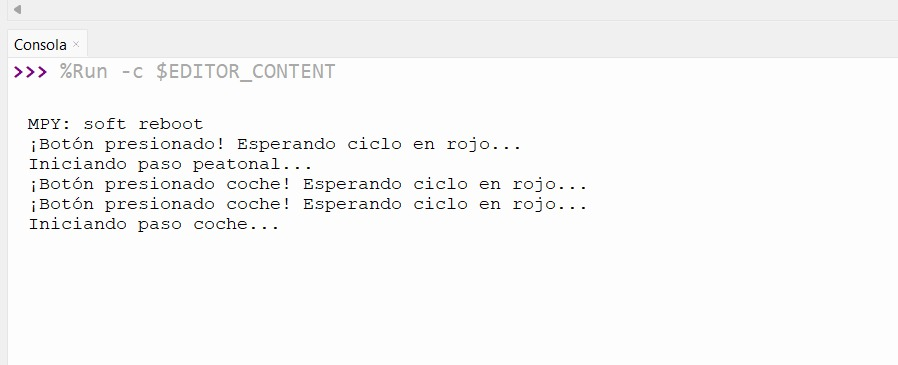
\includegraphics[width=0.75\textwidth]{img/Actividad6/Act6_0.jpg}
        \caption{Salida en consola mostrando las peticiones de botón peatonal y de coche, con los mensajes de inicio de paso.}
    \end{figure}

    \textbf{Primera interrupcion peaton:}

    \begin{figure}[H]
        \centering
        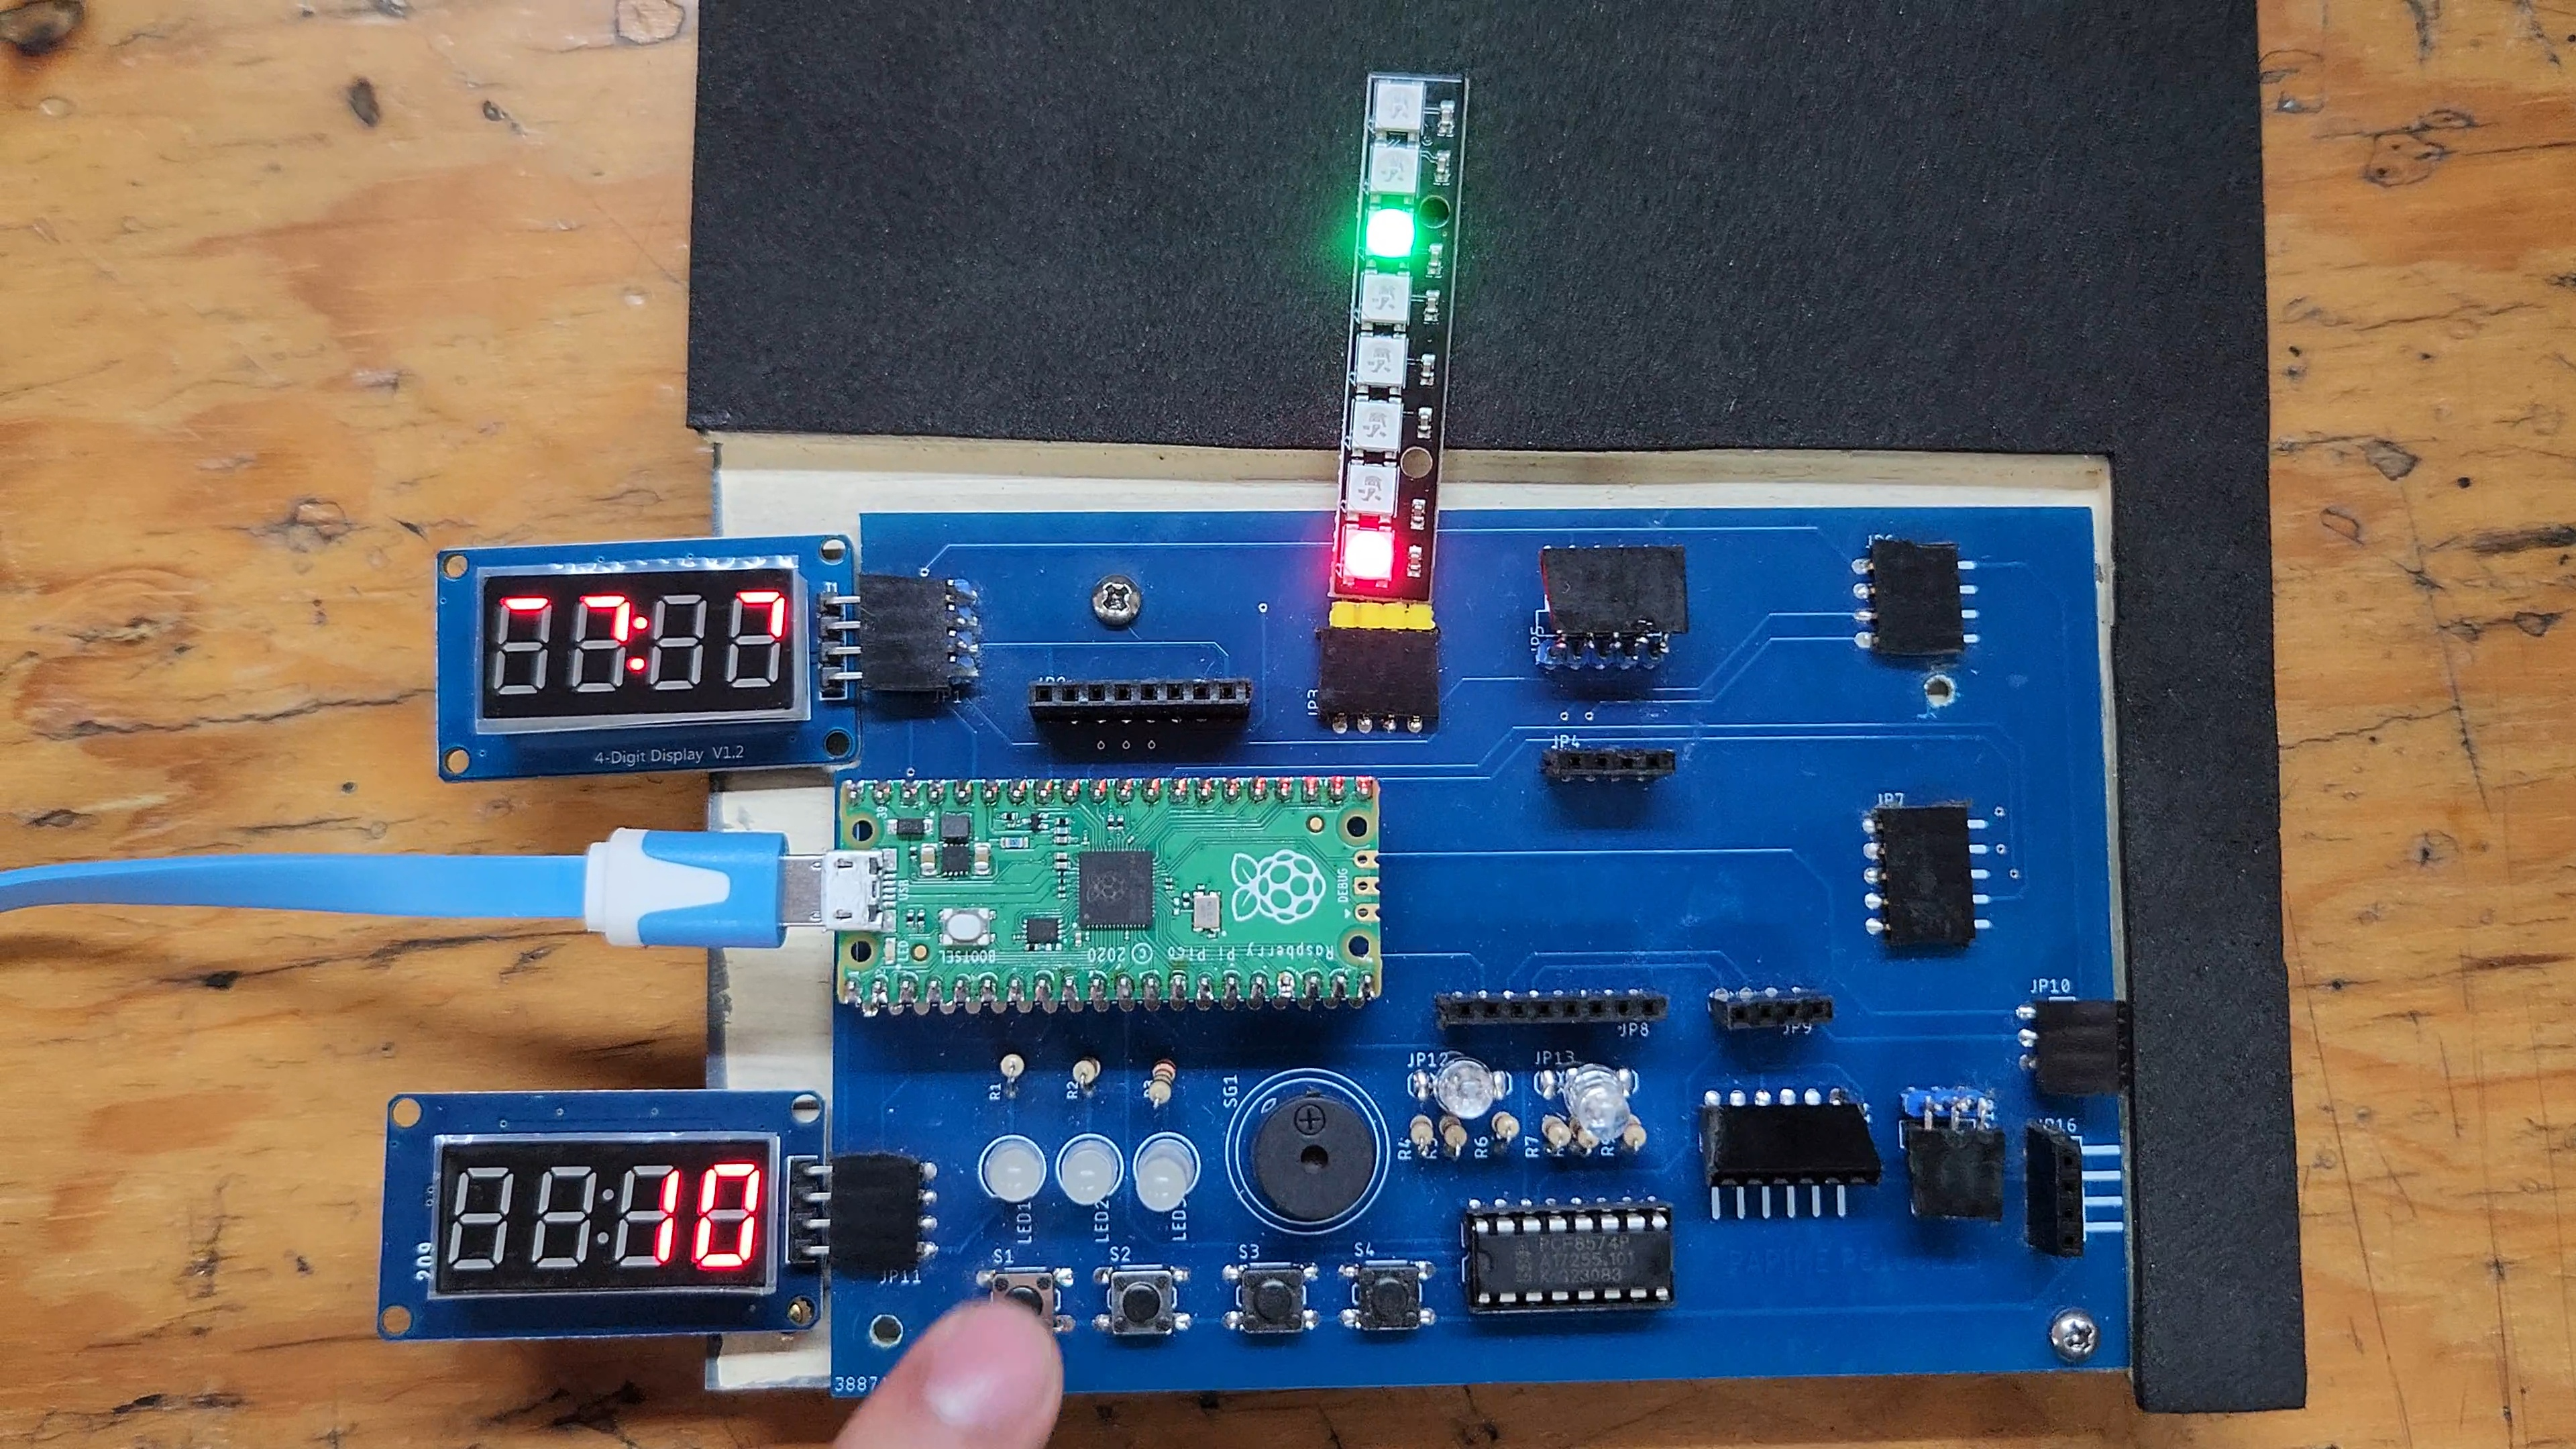
\includegraphics[width=0.75\textwidth]{img/Actividad6/Act6_1.jpg}
        \caption{Semáforo de autos en verde y peatón en rojo, display mostrando cuenta regresiva ``10'' durante paso de coches.}
    \end{figure}

    \begin{figure}[H]
        \centering
        
\includegraphics[width=0.75\textwidth]{img/Actividad6/Act6_9.jpg}
        \caption{Display TM1637 mostrando ``6'' durante la cuenta regresiva del paso peatonal con buzzer activo.}
    \end{figure}

    \begin{figure}[H]
        \centering
        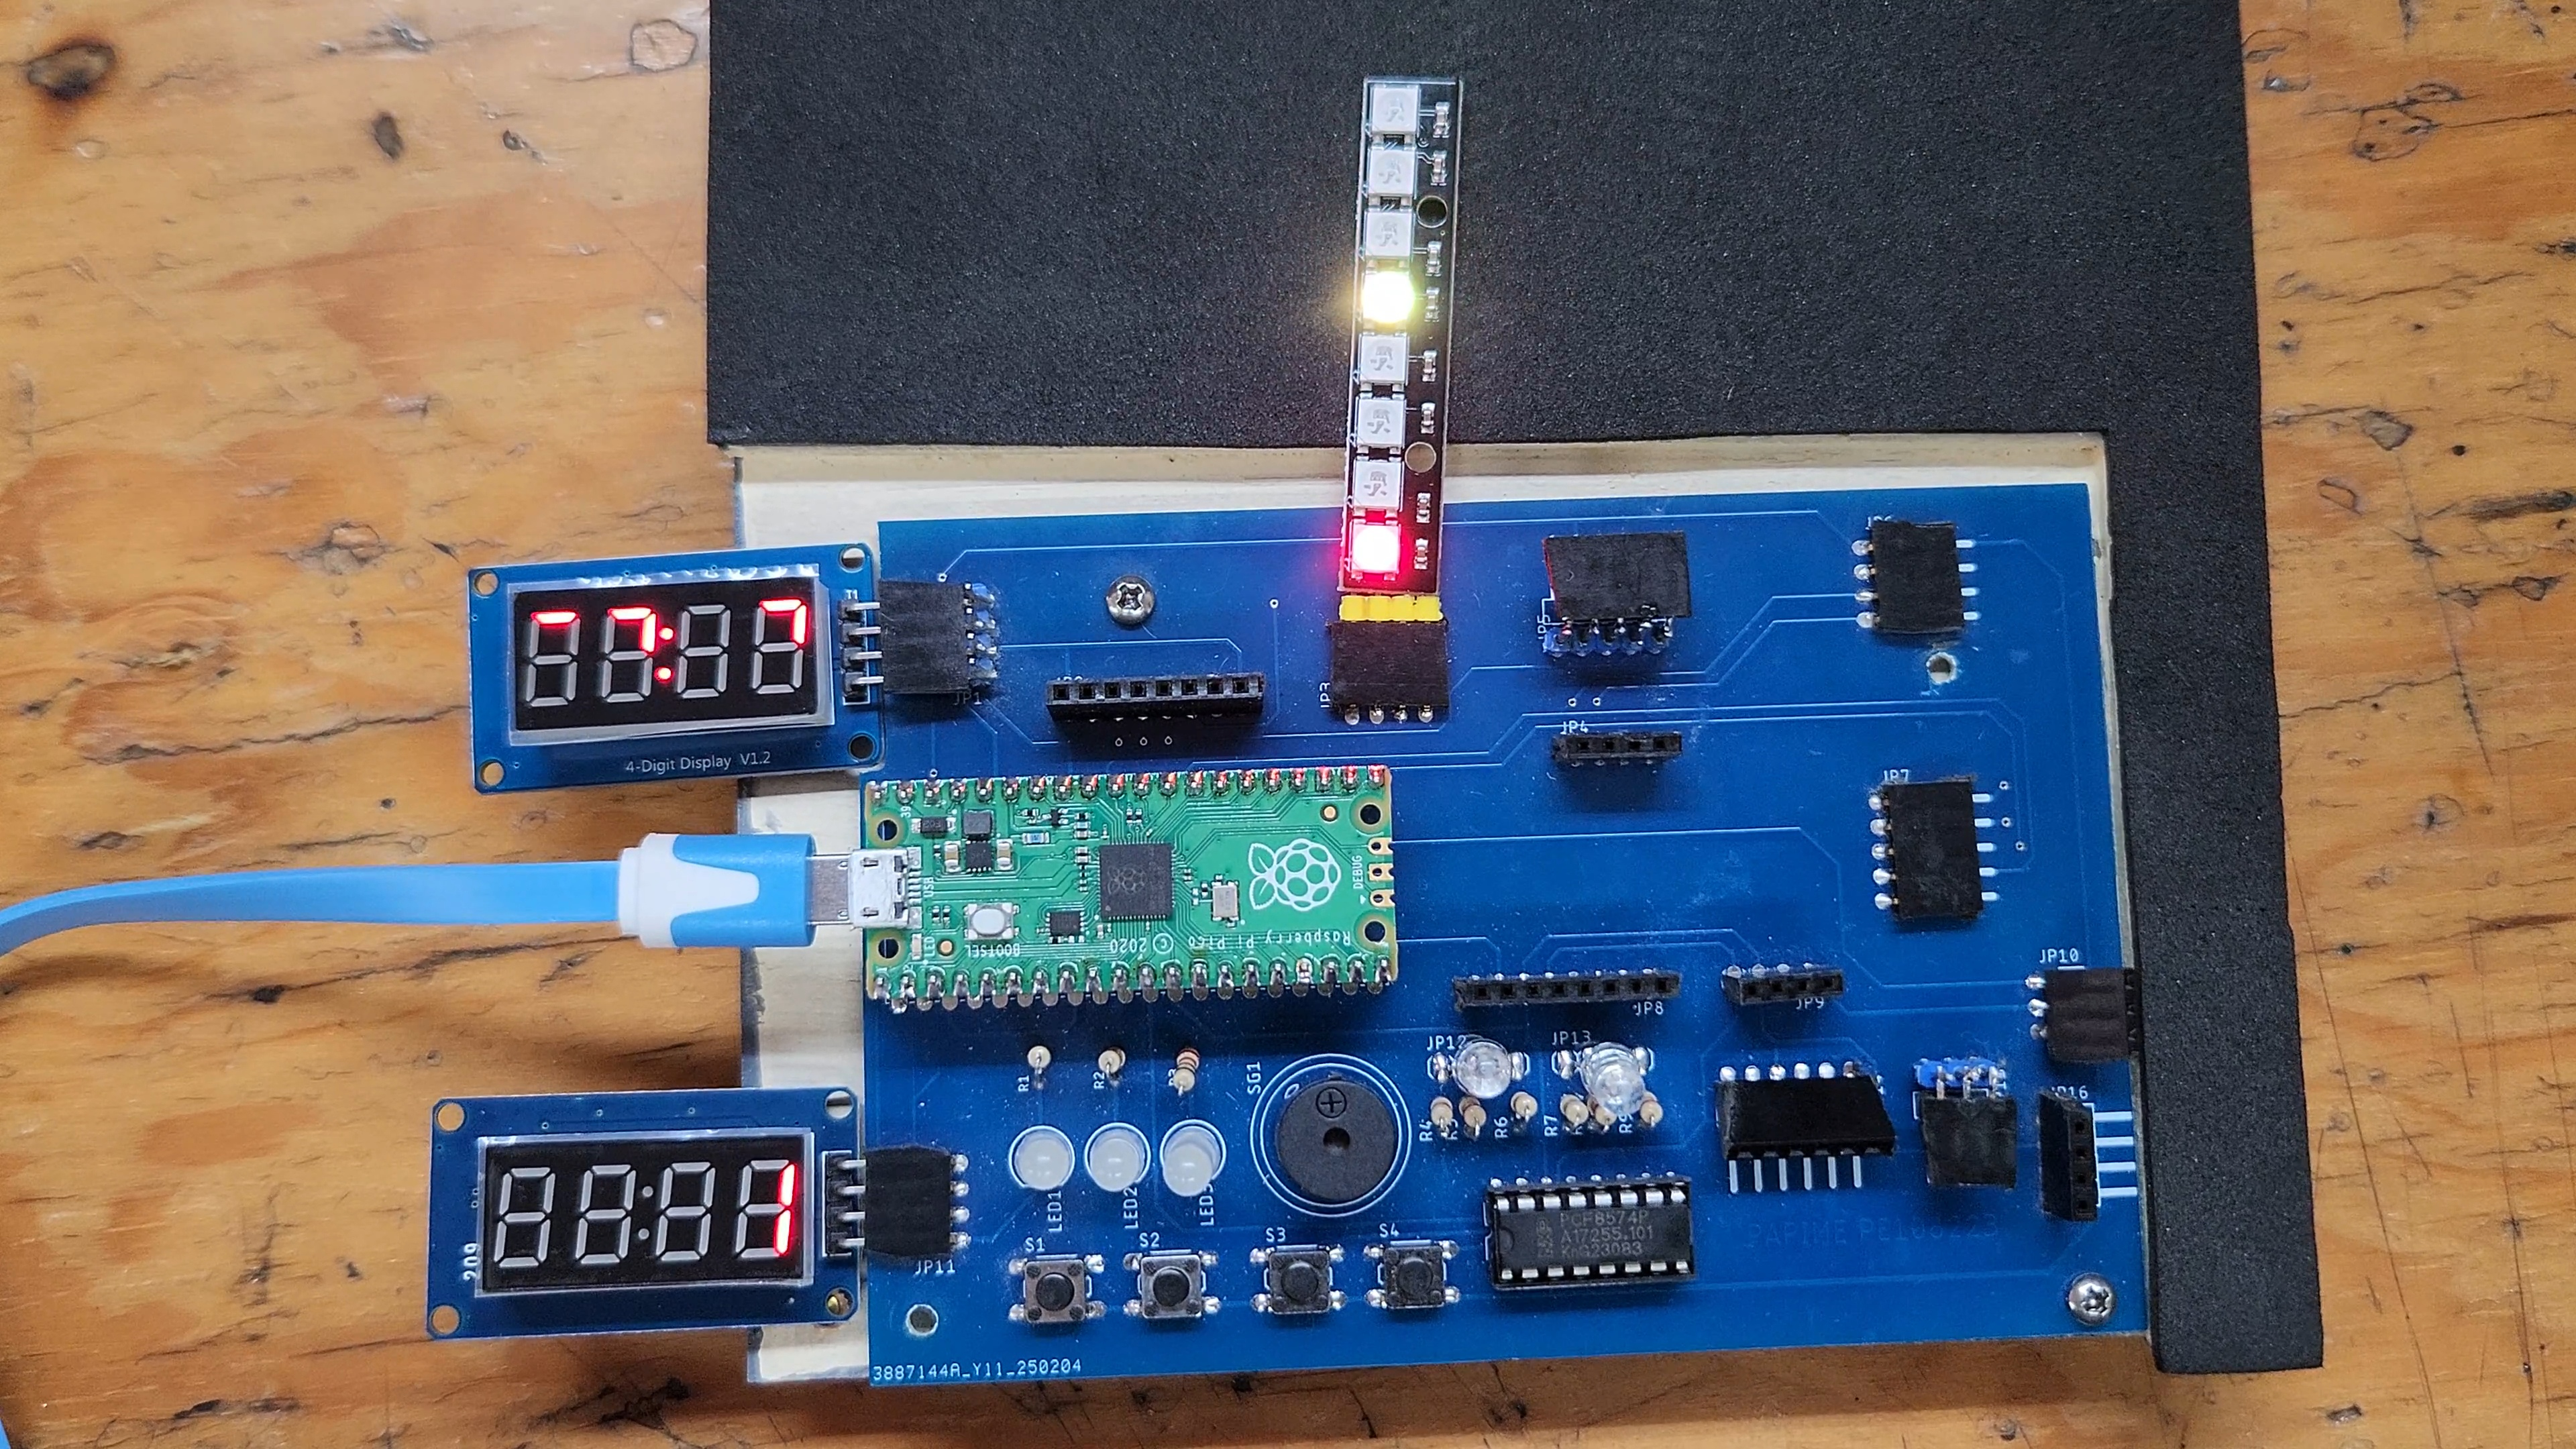
\includegraphics[width=0.75\textwidth]{img/Actividad6/Act6_3.jpg}
        \caption{Semáforo de autos en amarillo, transición antes de cambiar a rojo, peatón en rojo.}
    \end{figure}

    \begin{figure}[H]
        \centering
        
\includegraphics[width=0.75\textwidth]{img/Actividad6/Act6_4.jpg}
        \caption{Semáforo de autos en rojo y peatón con verde encendido, indicando cruce peatonal activo.}
    \end{figure}

    \begin{figure}[H]
        \centering
        
\includegraphics[width=0.75\textwidth]{img/Actividad6/Act6_5.jpg}
        \caption{Parpadeo de advertencia en amarillo para peatón, indicando que el tiempo de cruce está por terminar.}
    \end{figure}

    \begin{figure}[H]
        \centering
        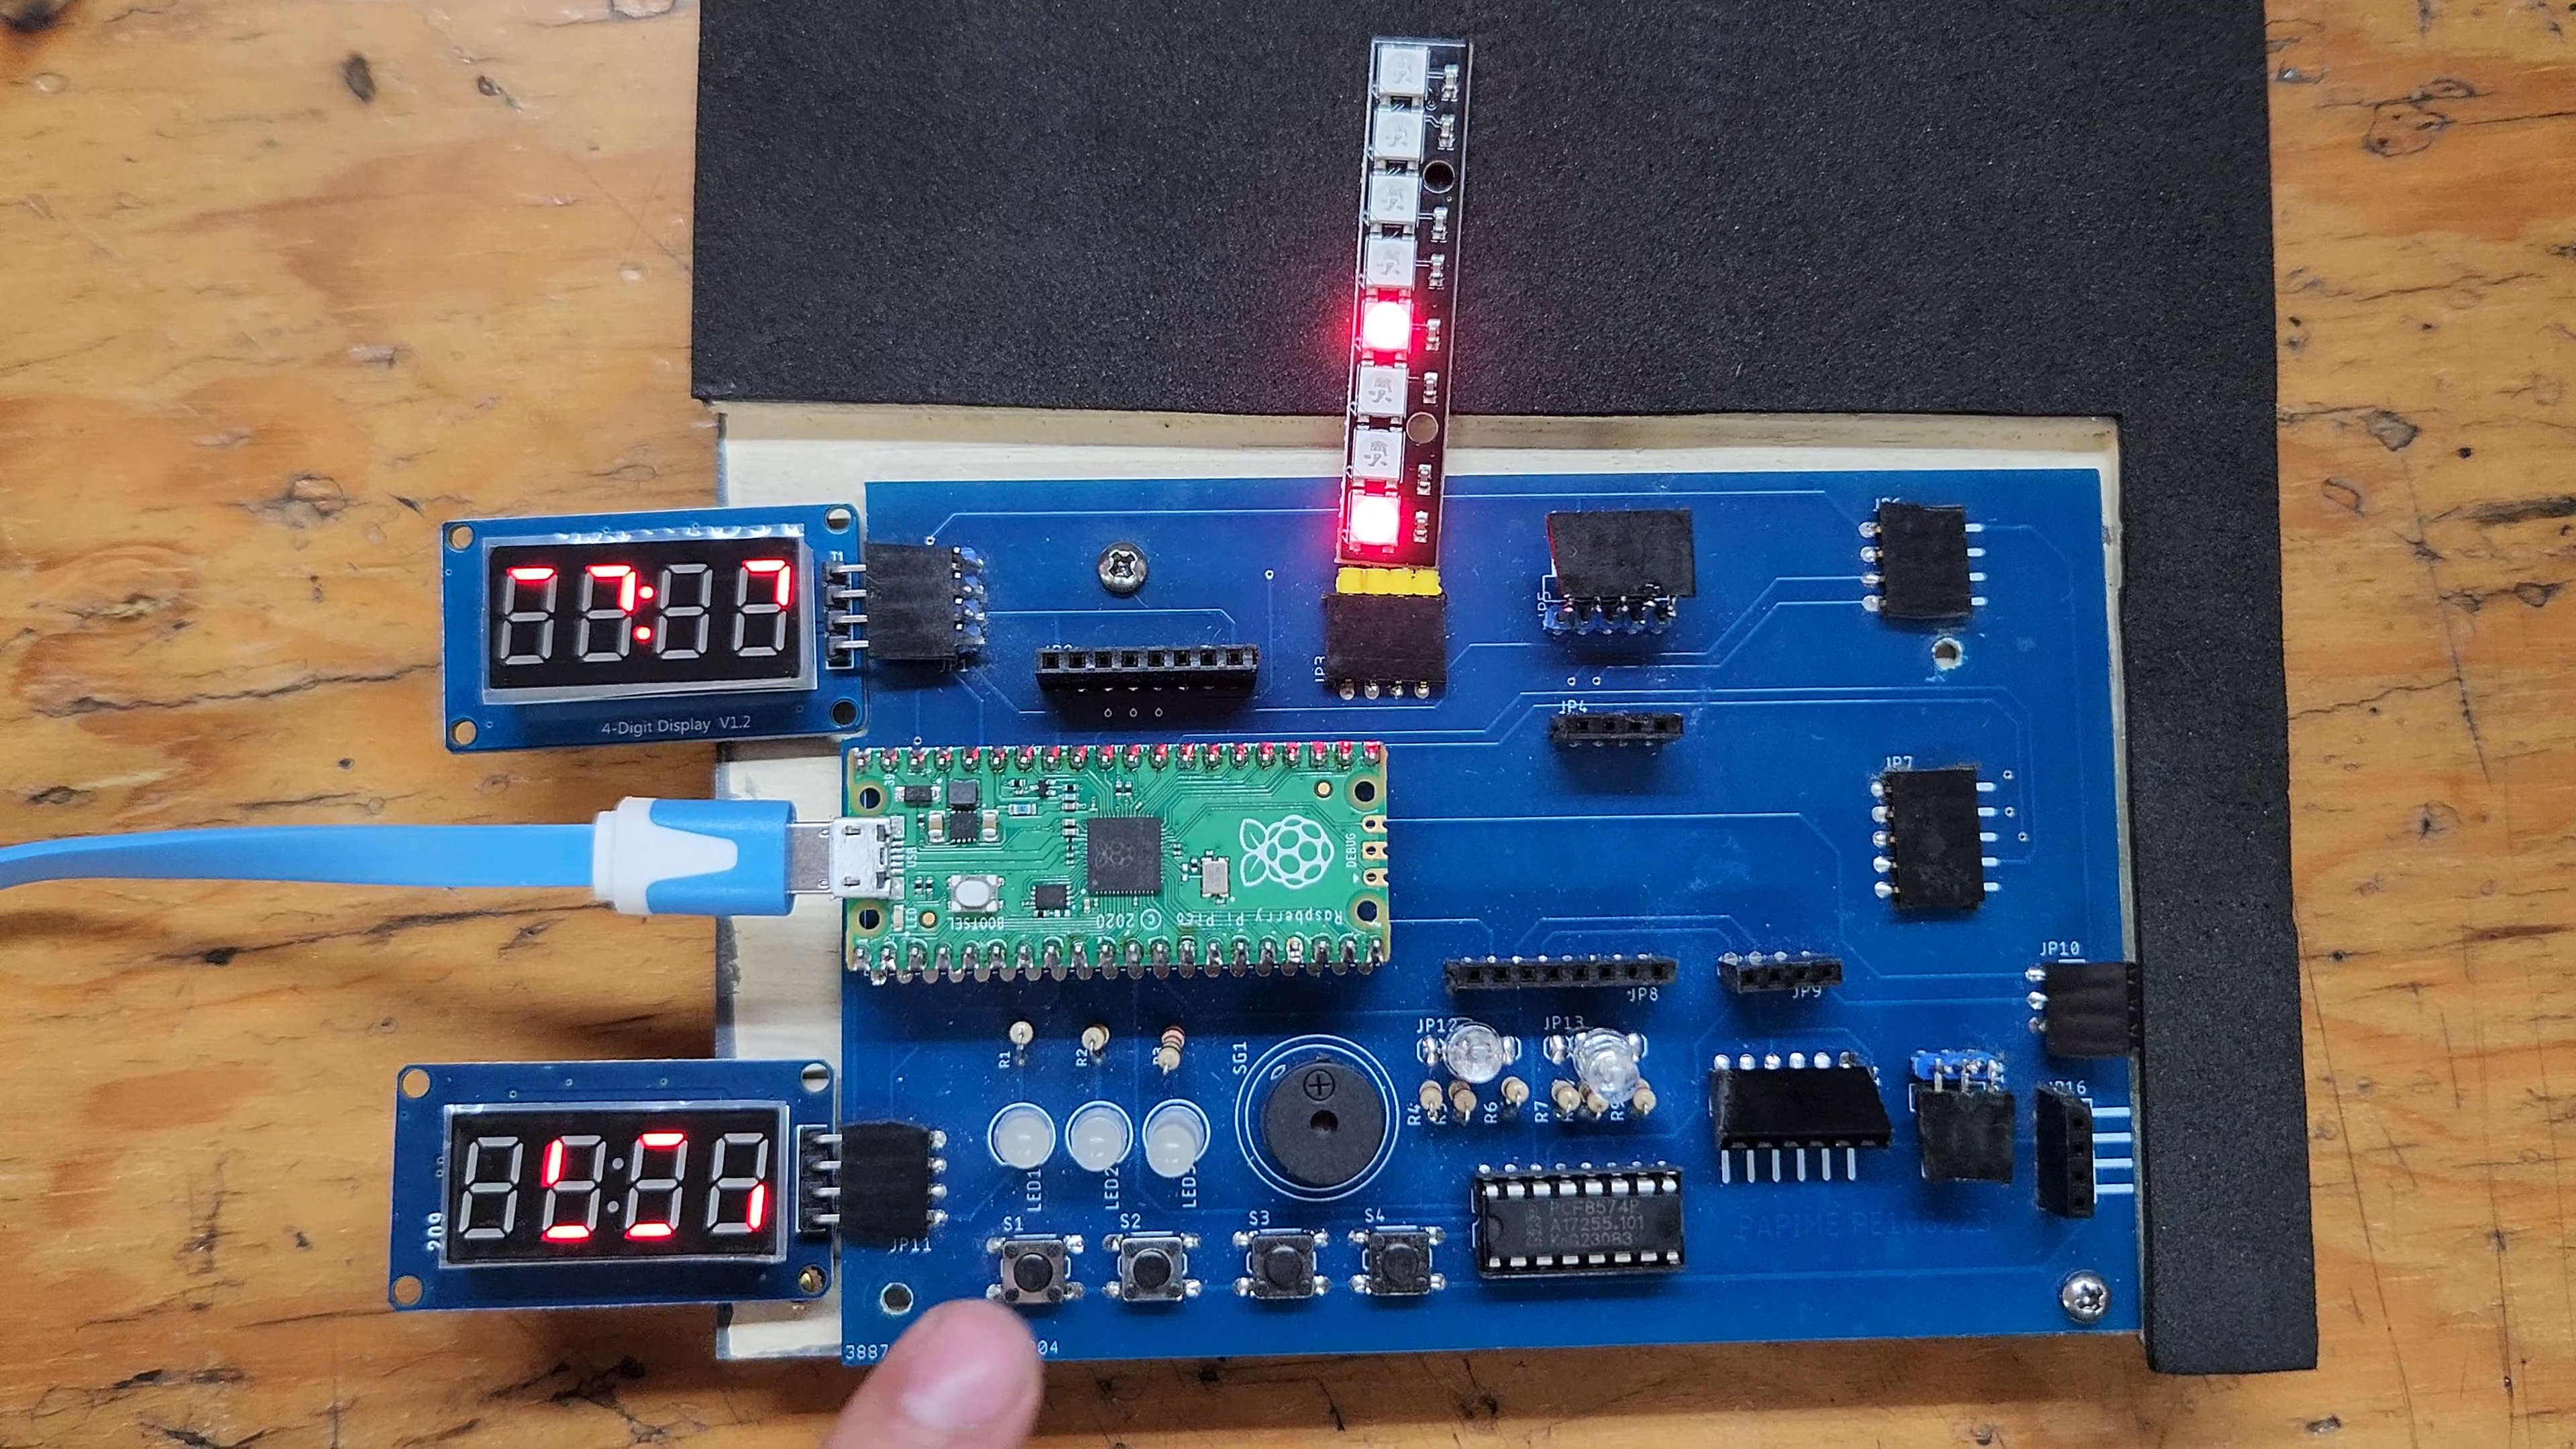
\includegraphics[width=0.75\textwidth]{img/Actividad6/Act6_14.jpg}
        \caption{Ambos semáforos en rojo, estado de transición entre ciclos del semáforo.}
    \end{figure}

    \textbf{Segunda interrupción coche:}

    \begin{figure}[H]
        \centering
        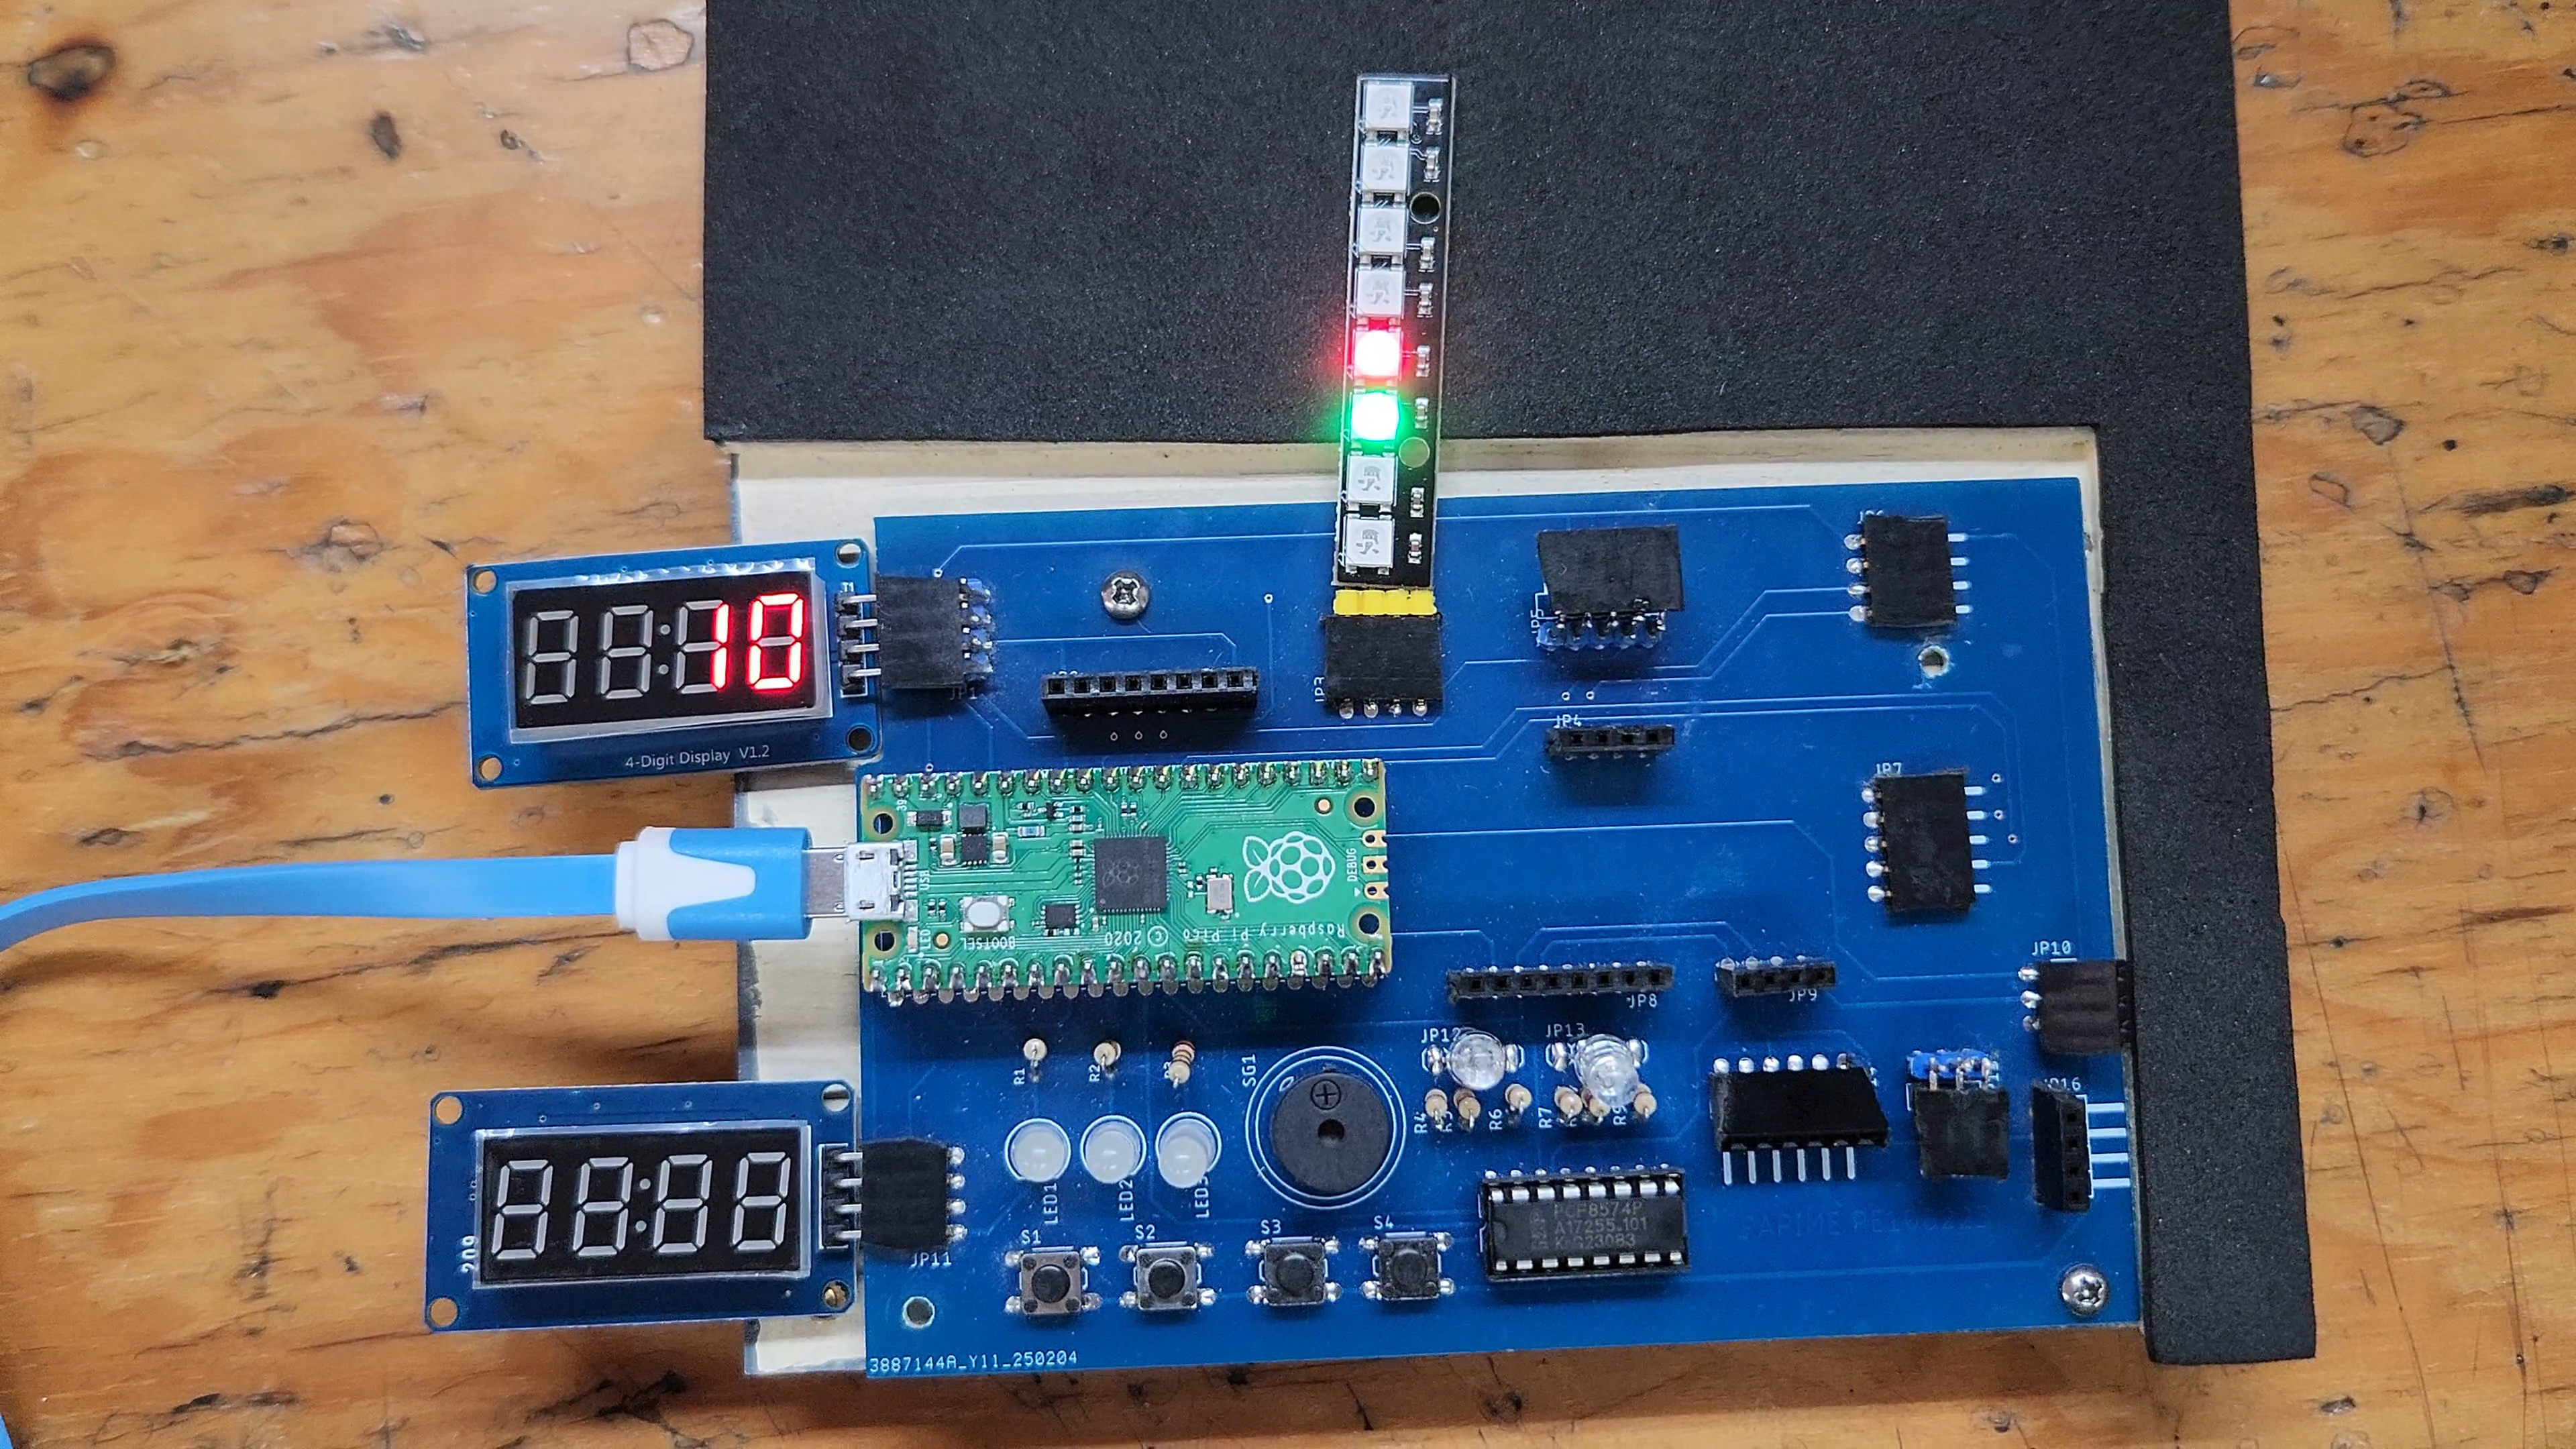
\includegraphics[width=0.75\textwidth]{img/Actividad6/imagen10.png}
        \caption{Semáforo de peaton en verde y auto en rojo, display mostrando cuenta regresiva ``10'' durante paso de peaton.}
    \end{figure}

    \begin{figure}[H]
        \centering
        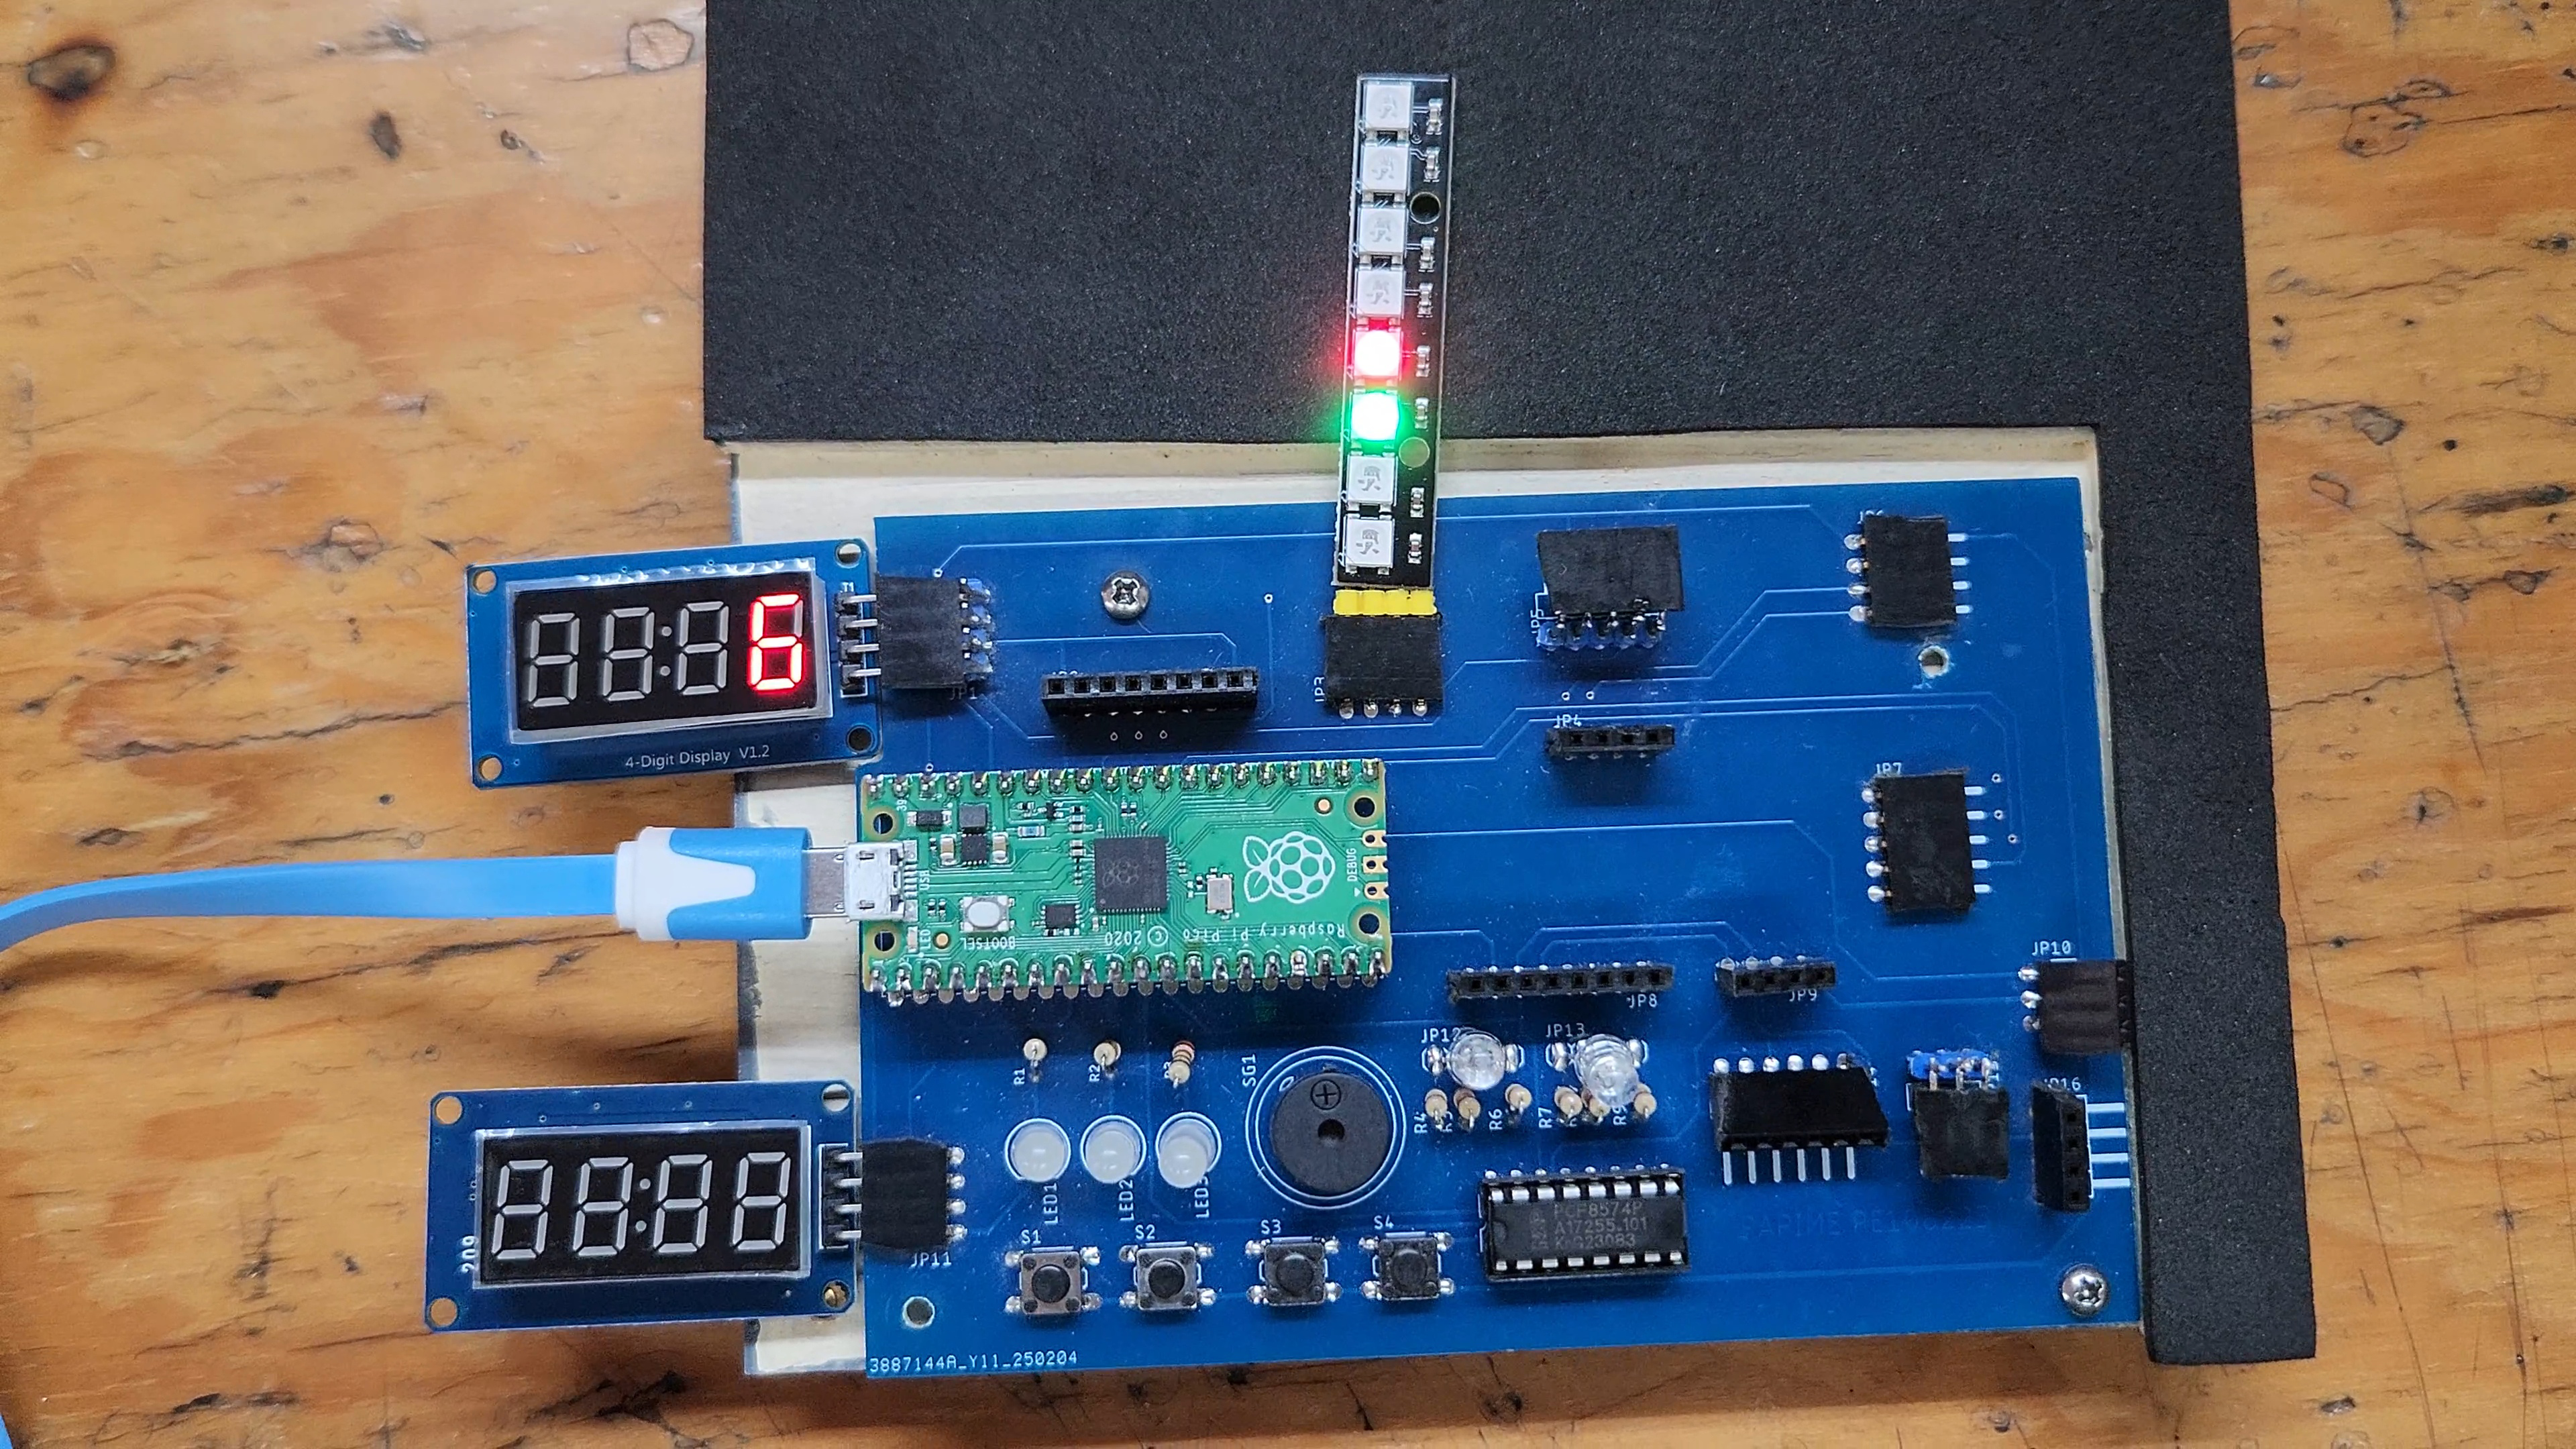
\includegraphics[width=0.75\textwidth]{img/Actividad6/image6.png}
        \caption{Display TM1637 mostrando ``6'' durante la cuenta regresiva del paso de los coches.}
    \end{figure}

    \begin{figure}[H]
        \centering
        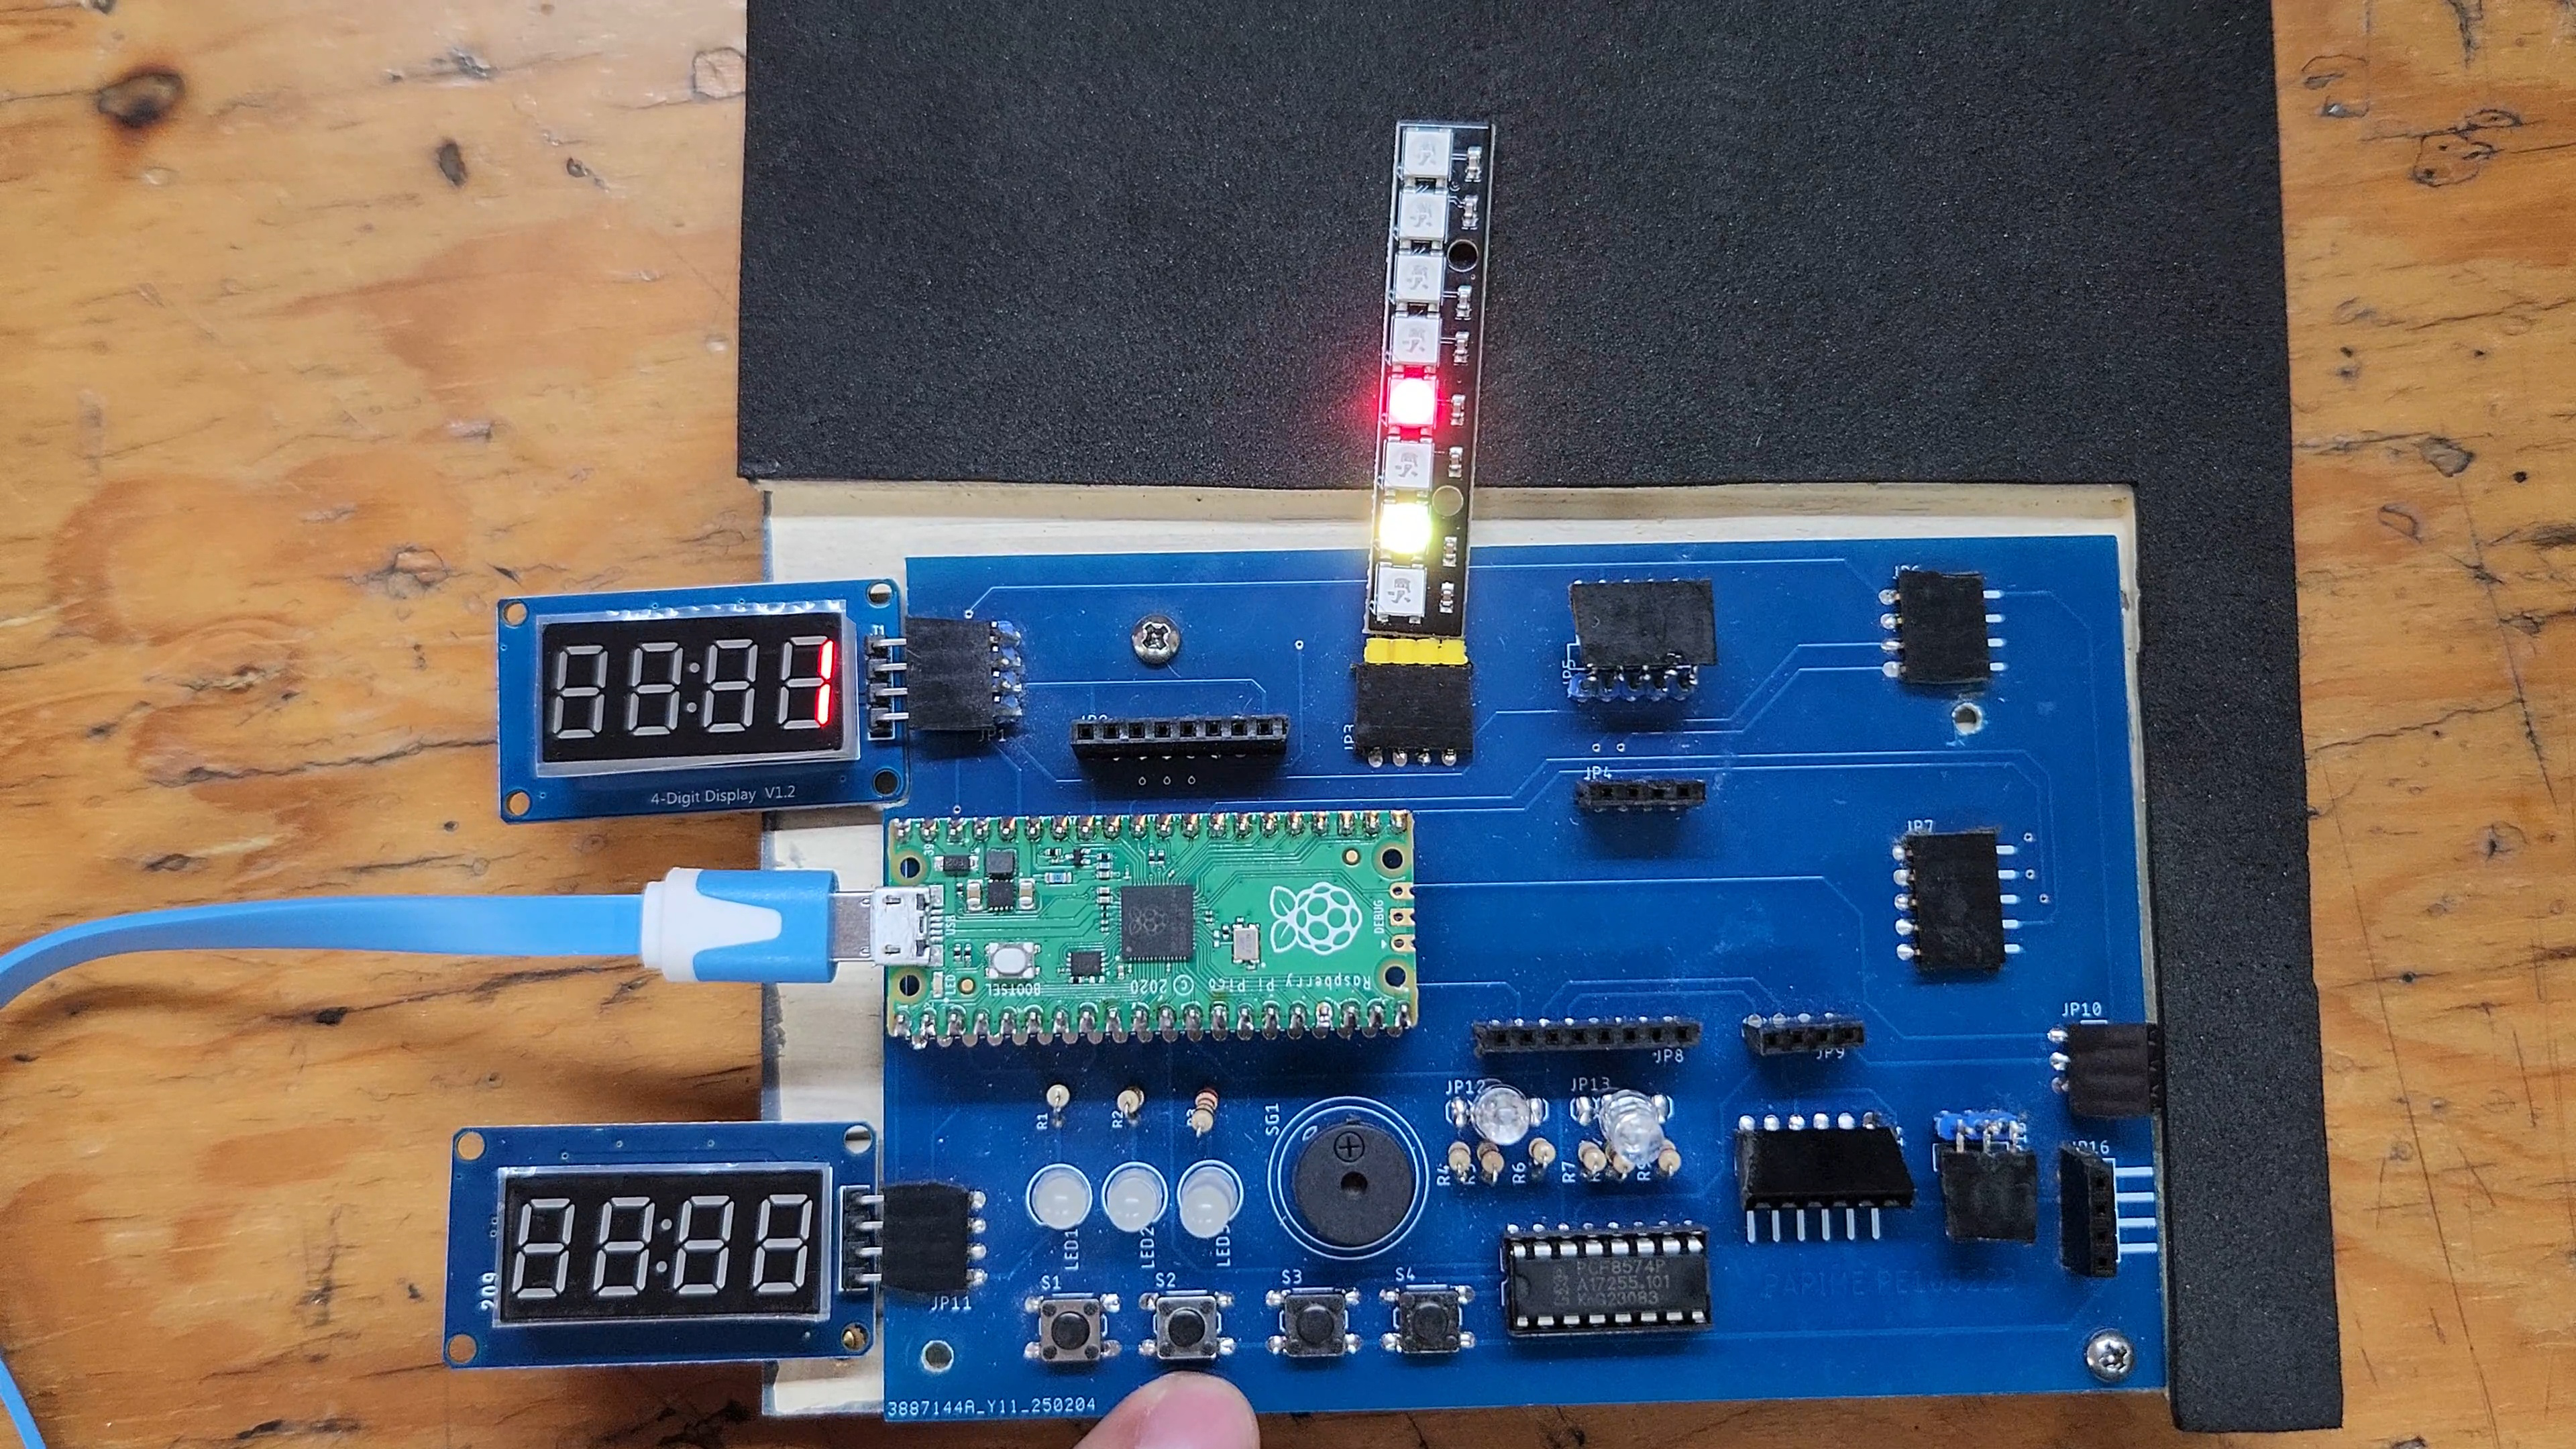
\includegraphics[width=0.75\textwidth]{img/Actividad6/image1.png}
        \caption{Semaforo en amarillo, a un segundo de cambiar el semaforo de peatones a verde.}
    \end{figure}

    \subsection*{Análisis de resultados}

    Los resultados obtenidos en la Actividad 6 demuestran el correcto funcionamiento de un sistema de semáforo inteligente que integra múltiples periféricos y aprovecha la arquitectura de doble núcleo del RP2040. Como se observa en la Figura 15, la consola serial registra adecuadamente los eventos de pulsación de botones y el inicio de los pasos peatonal y de coches, confirmando que las interrupciones por flanco de bajada configuradas en los pines GPIO12 y GPIO13 detectan correctamente las pulsaciones. En la Figura 16 se aprecia el semáforo de automóviles en verde (LED Neopixel índice 2) con el display TM1637 mostrando el valor ``10'' al inicio de la cuenta regresiva durante el paso de coches, mientras que el semáforo peatonal permanece en rojo (LED Neopixel índice 3), validando la correcta asignación de los índices de LEDs en la tira Neopixel. La Figura 17 muestra la transición a amarillo en el semáforo de autos, fase que dura 2 segundos según la programación, lo cual coincide con el comportamiento esperado del ciclo normal controlado por el Núcleo 0. La Figura 18 evidencia el momento en que se activa el cruce peatonal: el semáforo de autos muestra rojo y el peatonal enciende en verde, confirmando que el mecanismo de sincronización mediante el lock funciona correctamente, ya que el Núcleo 1 adquiere el lock e impide que el Núcleo 0 cambie el estado del semáforo de autos durante el cruce. En la Figura 19 se observa el parpadeo de advertencia en amarillo para el peatón, secuencia que se ejecuta tres veces antes de regresar a rojo peatonal, alertando al peatón de que el tiempo de cruce está por finalizar. La Figura 20 muestra el display TM1637 durante la cuenta regresiva con el valor ``8'', acompañada de la señal acústica del buzzer que emite un tono de 1000 Hz durante 200 ms por cada segundo, proporcionando retroalimentación auditiva al peatón. La Figura 21 confirma que la cuenta regresiva se despliega correctamente mostrando ``9'' al inicio del paso de coches. Finalmente, la Figura 22 muestra ambos semáforos en rojo durante el estado de transición, momento en el que el Núcleo 0 libera el lock y espera 50 ms para dar oportunidad al Núcleo 1 de adquirirlo si existe una petición pendiente. La implementación demuestra un uso efectivo de las interrupciones de hardware para mantener las ISR breves (solo activan banderas), la sincronización entre núcleos mediante locks para evitar condiciones de carrera, y la coordinación de múltiples periféricos (Neopixel, TM1637, PWM para buzzer) en un sistema embebido de tiempo real.

    \section{Conclusiones:}

    \begin{itemize}
        \item \textbf{Espinoza Matamoros Percival Ulises:} A partir de la implementación de esta práctica, logré comprender de manera más extensa el funcionamiento de las interrupciones e hilos en los programas para la Raspberry Pi Pico. De forma que por medio de las interrupciones, el programa puede responder de manera inmediata a eventos externos, como la pulsación de un botón, sin necesidad de detener o bloquear el flujo principal del programa. Por otro lado el uso de hilos permite ejecutar tareas concurrentes en ambos núcleos de la tarjeta, de forma que se pueden implementar programas con múltiples funcionalidades que se ejecutan al mismo tiempo sin interferir entre sí, por lo que esto ofrece una perspectiva más amplia sobre las aplicaciones y posibilidades de programación microcontroladores. Por lo que a partir de la realización de esta práctica pude comprender dos conceptos fundamentales para el desarrollo de programas más complejos y eficientes en la Raspberry Pi Pico.

        \item \textbf{Flores Colin Victor Jaziel:} En esta práctica número once logre comprender de manera mas profunda el funcionamiento de las interrupciones y su aplicacion en sistemas de control en tiempo real con la Raspberry Pi Pico, ya que en las actividades en las que se implementó alguna especie de boton como S1, se usaba el disparador de interrupcion por flanco de bajada, pude observar como la pico responde de forma inmediata a un evento externo sin necesidad de estar revisando constantemente el estado del pin mediante sondeo, lo que optimiza el uso de recursos.

        Además con ayuda de la Raspberry Pi Pico implementamos actividades con dos botones S1 y S2, cada uno dispara su propia interrupcion por flanco de bajada activando acciones especificas (LEDs y contadores en TM1637) sin interferencias y el uso de 2 botones sirvió para dejar en claro el uso de hilos para ejecutar tareas concurrentes en ambos nucleos, como el control independiente del semaforo para autos y peatones con sincronizacion mediante locks, integrando interrupciones y multitarea en sistemas de control robustos.

        \item \textbf{Lara Hernandez Angel Husiel:} En esta práctica logré comprender de forma más clara cómo empezar a utilizar la Raspberry Pi Pico programando desde cero en MicroPython. Al trabajar con los diferentes componentes, como el display TM1637, la tira de LEDs NeoPixel y el buzzer, entendí mejor cómo manejar las entradas y salidas, así como la forma de generar señales PWM para los sonidos.
        También me quedó mucho más claro el uso de las interrupciones para los botones, ya que gracias a ellas el programa puede responder al instante cuando alguien presiona un botón, sin necesidad de trabar o frenar todo el código. Por otro lado, usar los dos núcleos de la tarjeta al mismo tiempo fue algo nuevo; aprendí que usando hilos y los "locks" puedo hacer que el semáforo normal siga funcionando y al mismo tiempo escuchar las peticiones de los peatones sin que haya problemas. 
    \end{itemize}

    \newpage


    \nocite{*} 
    \printbibliography[heading=bibintoc, title={Referencias}]

\end{document}